\chapter{\label{appendix}Appendix}



\section{Data Reduction using Exploratory Factor Analysis} \label{appendix:EFA}
EFA is one of various available data reduction techniques, and is distinct from its main alternative, Principal Components Analysis (PCA), in that it is capable of modelling the latent dimensions of a collection of variables.\footnote{PCA is concerned only with establishing which components exist within the existing data and how a particular variable might contribute that component. To do this, PCA makes the assumption that all variance in a subset of variables is common variance, and therefore communality between all variables is equal to 1. From this assumption, the original data can be transposed into a linear model without the need for a communality-dependent estimated coefficient for each variable \citep{Widaman2007}. EFA examines all the pairwise relationships between individual variables and seeks to extract latent factors from the measured variables.  Squared Multiple Correlations (which are essentially multiple regressions in which each variable is predicted by all others) were used to calculate the common variance (communality) between each variable in an analysis (the communality value is much like an R-squared value from a multiple regression).
The square root of the communality score for each variable is then used as a coefficient that conditions the relationship between each variable and the underlying dimensions (factors) identifiable in the data. Also known as ``factor loadings,'' these coefficients become the parameters of linear model capable of estimating factor scores for each individual observation, which can be utilised in subsequent statistical analysis in place of single variable observations.

A final step in the EFA procedure is the process of ``rotation'', which is an optimisation technique designed to encourage each variable to load on as few factors as possible \citep{Rummel1988}. Rotation refers to a geometric conception of factor analysis, in which individual variables can be plotted in n-dimensional space according to their relationship to each dimension (factor). By rotating the axes of these dimensions, the distance of a given variable to that dimension can be reduced, which results in an increase in factor loading on one factor and (ideally) a decrease in factor loading on another uncorrelated variable. Orthogonal (or perpendicular) rotation of axes refers to axes, say X and Y, maintaining a 90-degree perpendicularity and rotating clockwise or anticlockwise, depending on the location of the variable clusters.
Orthogonal rotation thus enables optimisation of loadings for clusters of variables that are distant from each other in n-dimensional space. If correlation exists between clusters of variables, however, rotating axes obliquely (inwards towards each other) provides a more effective way of reducing the distance between clusters of variables and the latent dimensions that account for such clustering \citep{Osborne2015}. See Figure ~\ref{fig:orthogonalOblique} for a graphical  illustration of the difference between orthogonal and oblique rotation. Given that most variables of interest in the present study were correlated to some degree, I opted for an oblique rotation method \citep{Field2012}. EFAs were conducted using the factanal() function in the Stats package (Version 3.3.0) in R, using the ``promax'' (oblique) rotation method \citep{Gorsuch1983}. Factor scores were standardised z-scores: zero-centred, with a standard deviation of 1.

\begin{figure}[htbp]
  \begin{center}
    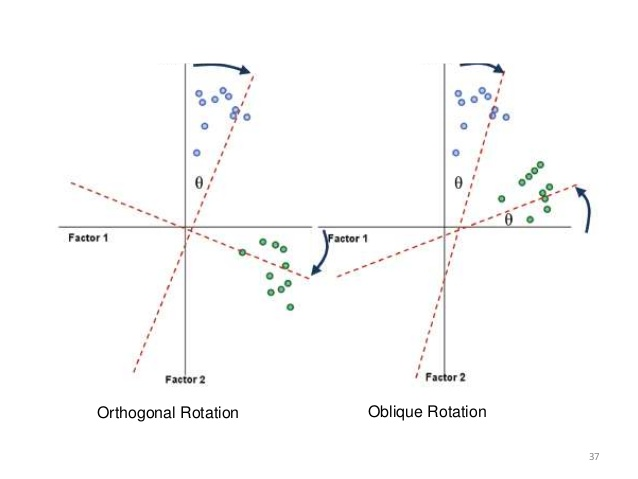
\includegraphics[width= \linewidth, scale = .5]{images/orthogonalObliqueRotationExample.jpg}
    \caption{Orthogonal and oblique rotation methods}
    \label{fig:orthogonalOblique}
  \end{center}
\end{figure}






\section{}


\begin{figure}[htbp]
    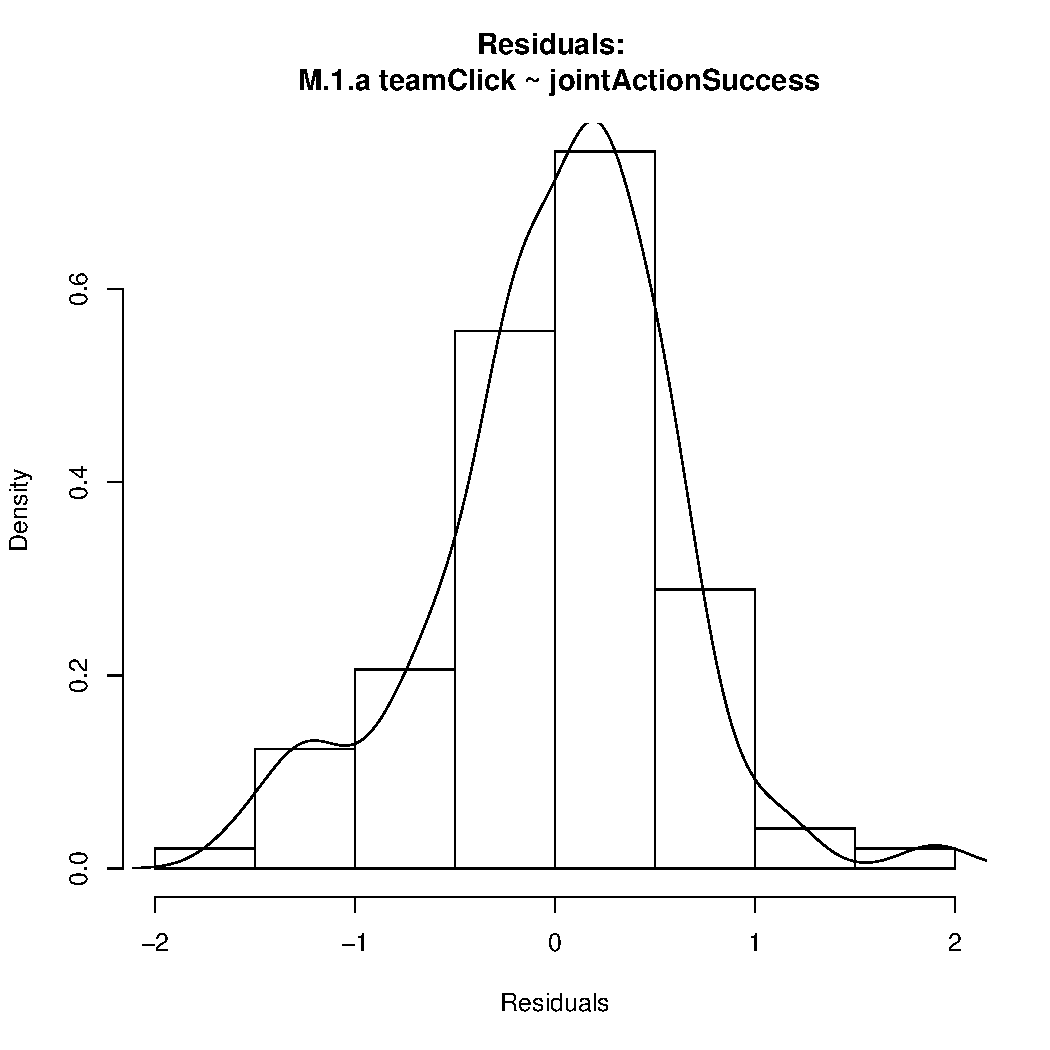
\includegraphics[scale =.4]{images/MLM1aHist.pdf}
    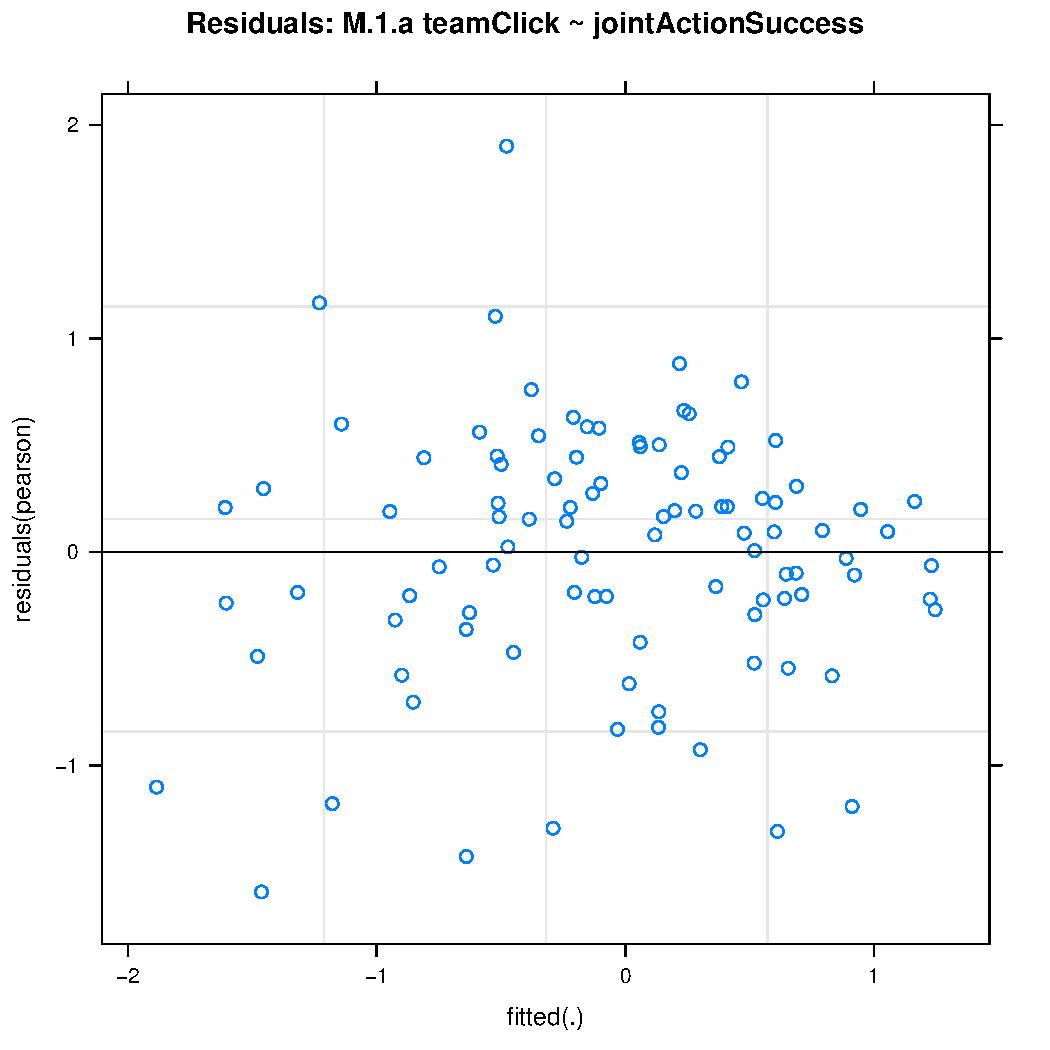
\includegraphics[scale =.4]{images/MLM1aScatter.pdf}
    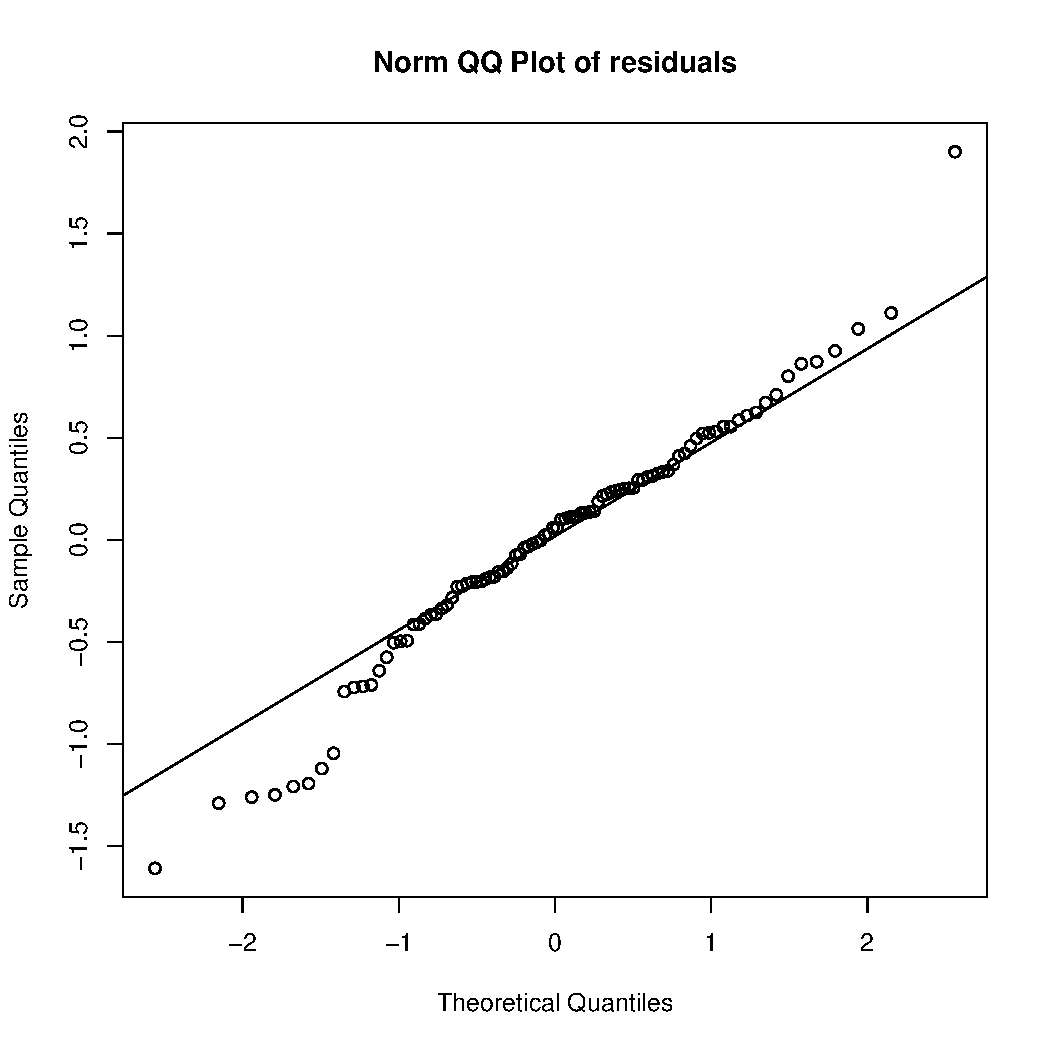
\includegraphics[scale =.4]{images/MLM1aQQPlot.pdf}
    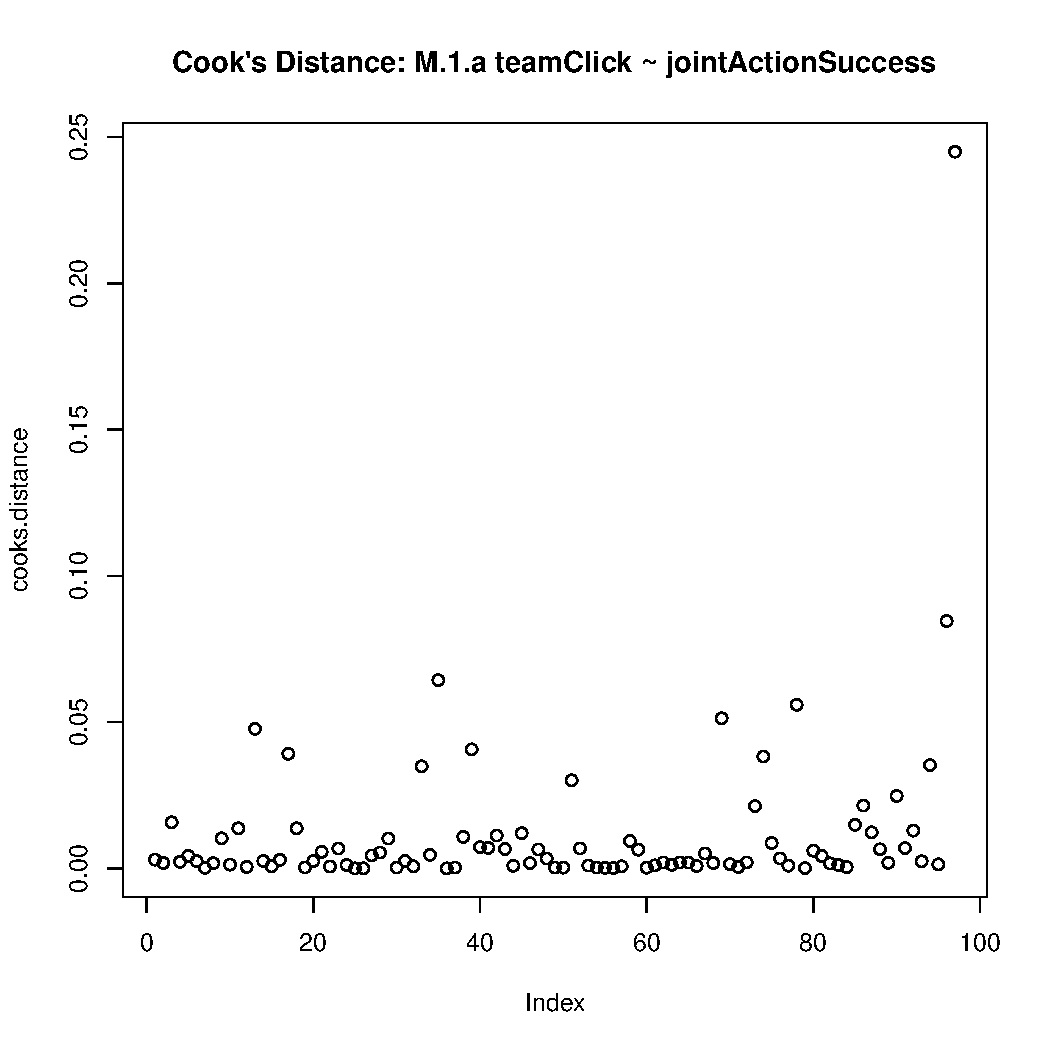
\includegraphics[scale =.4]{images/MLM1aCooksD.pdf}
    \caption{Model Assumptions: 1.a Joint Action Success Predicts Team Click}
    \label{fig:MLM1aAssumptions}
\end{figure}





\begin{figure}[htbp]
  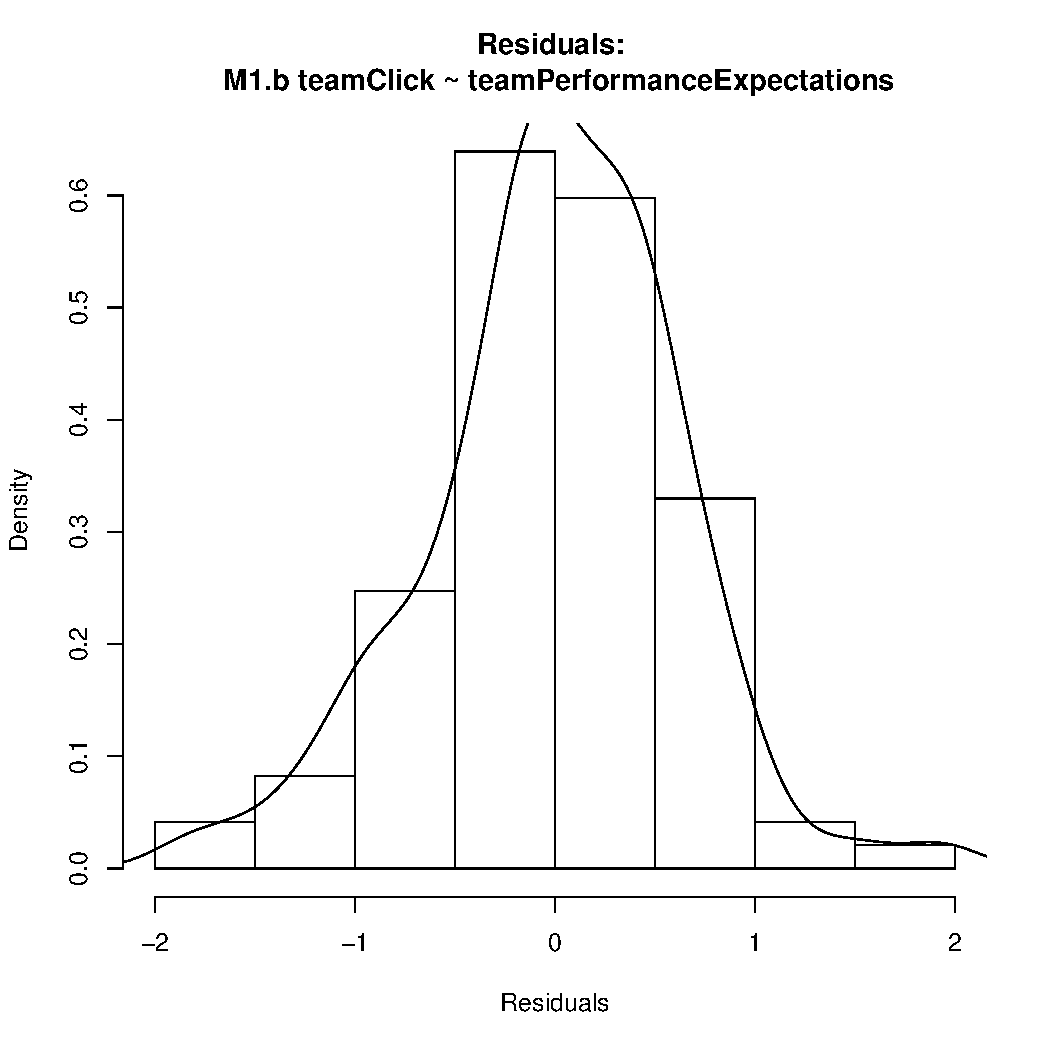
\includegraphics[scale =.4]{images/MLM1bHist.pdf}
  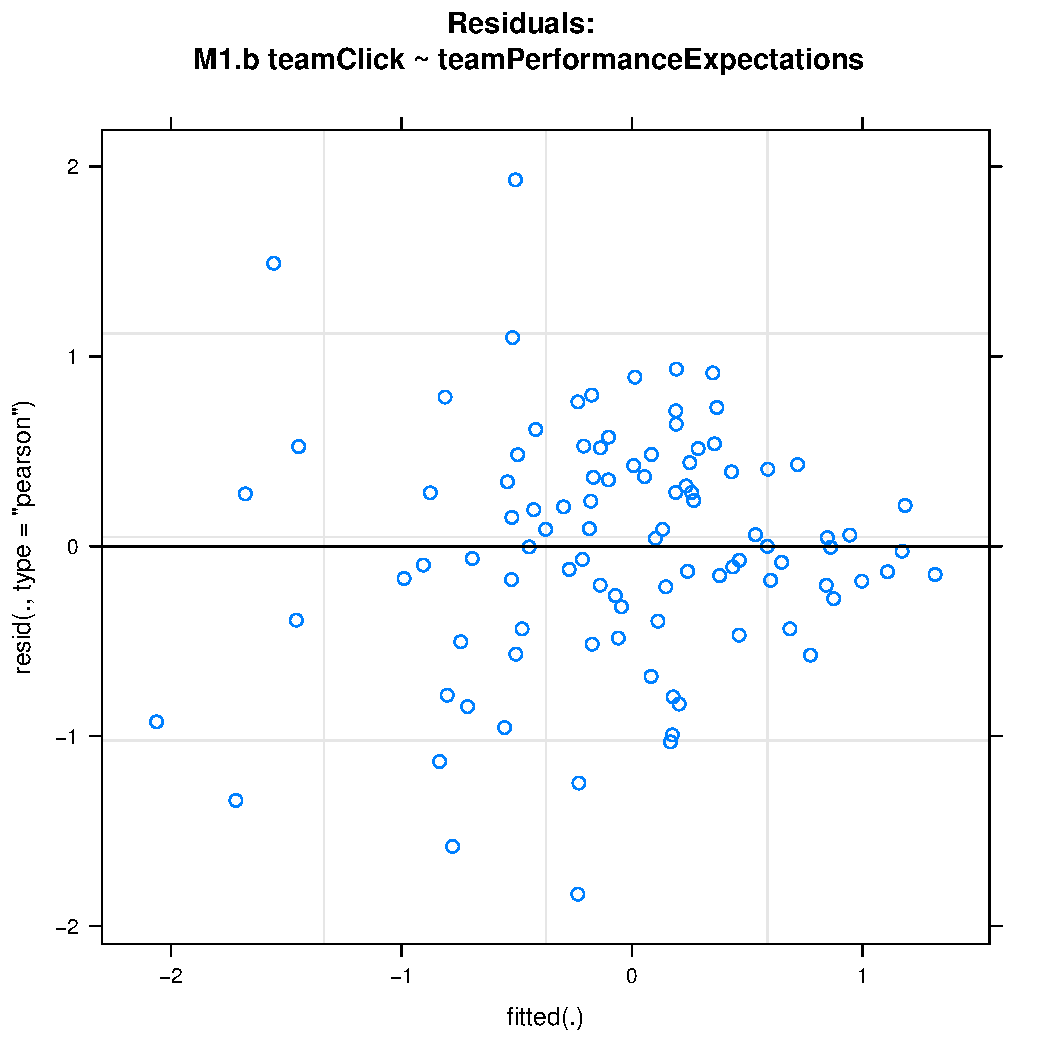
\includegraphics[scale =.4]{images/MLM1bScatter.pdf}
  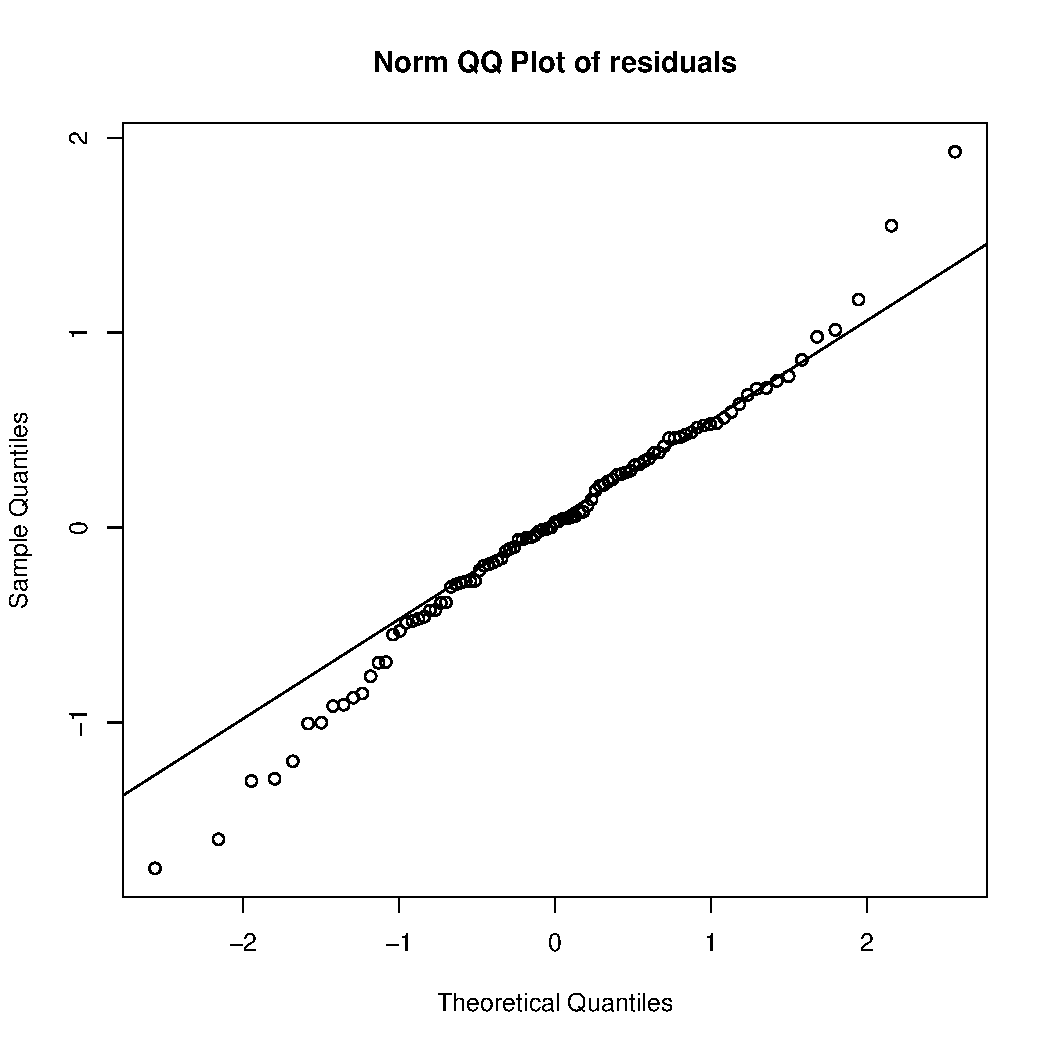
\includegraphics[scale =.4]{images/MLM1bQQNorm.pdf}
  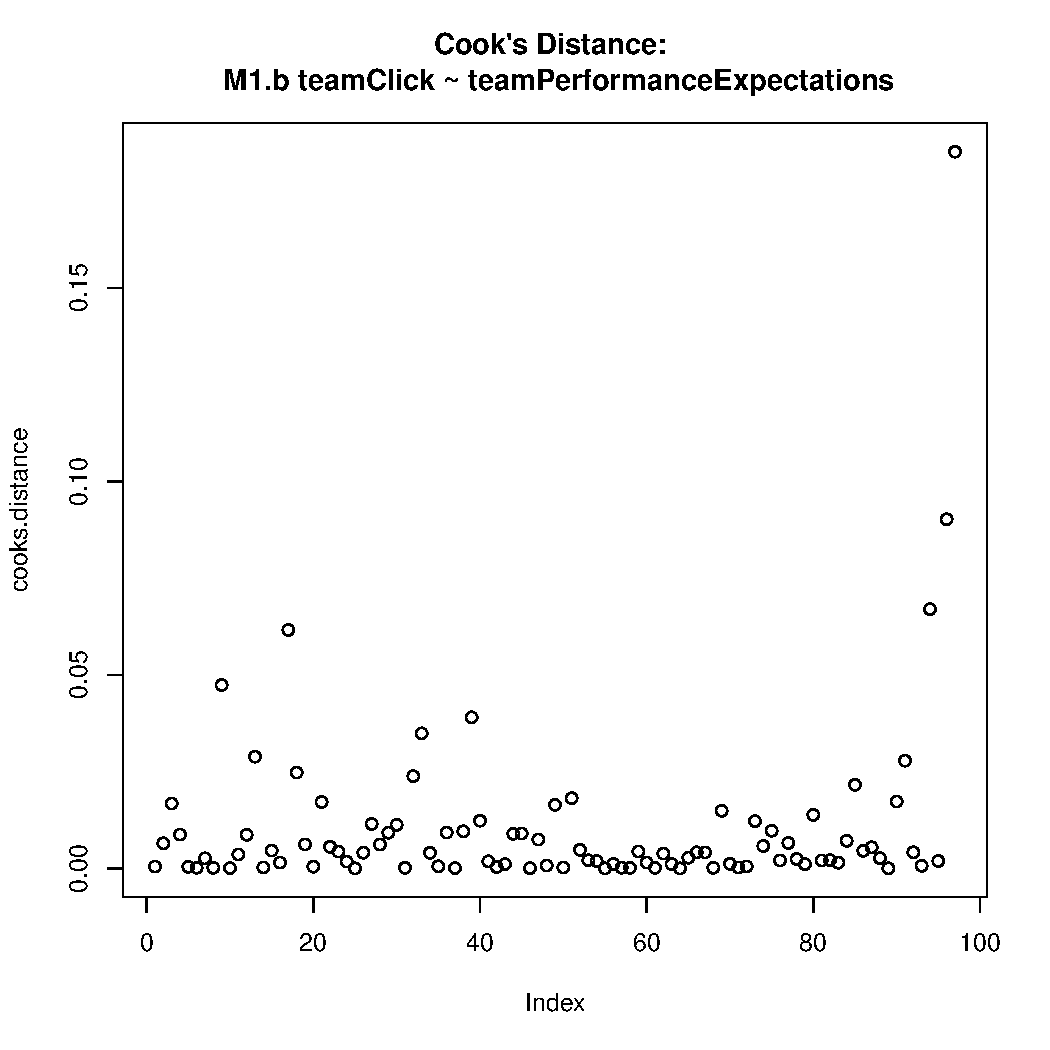
\includegraphics[scale =.4]{images/MLM1bCooksD.pdf}
  \caption{Model Assumptions: Model 1b Team Performance Expectations predict Team Click}
  \label{fig:MLM1bAssumptions}
\end{figure}





% Table created by stargazer v.5.2 by Marek Hlavac, Harvard University. E-mail: hlavac at fas.harvard.edu
% Date and time: Mon, Jun 26, 2017 - 20:35:23
\begin{table}[!htbp] \centering 
  \caption{teamClick = jointActionSuccess X teamPerformanceExpectations} 
  \label{tab:MLM1cPerformanceClickInteraction} 
\footnotesize 
\begin{tabular}{@{\extracolsep{5pt}}lc} 
\\[-1.8ex]\hline 
\hline \\[-1.8ex] 
 & \multicolumn{1}{c}{\textit{Dependent variable:}} \\ 
\cline{2-2} 
\\[-1.8ex] & teamClick \\ 
\hline \\[-1.8ex] 
 (constant) & $-$0.83$^{*}$ \\ 
  & (0.41) \\ 
  & \\ 
 jointActionSuccess & 0.57$^{*}$ \\ 
  & (0.25) \\ 
  & \\ 
 teamPerformanceExpectations & 0.01 \\ 
  & (0.005) \\ 
  & \\ 
 indPerformanceSuccess & 0.01 \\ 
  & (0.10) \\ 
  & \\ 
 indPerformanceExpectations & $-$0.001 \\ 
  & (0.003) \\ 
  & \\ 
 objectiveCompetence & 0.06 \\ 
  & (0.08) \\ 
  & \\ 
 subjectiveCompetence & 0.10 \\ 
  & (0.07) \\ 
  & \\ 
 finalRank & 0.03 \\ 
  & (0.04) \\ 
  & \\ 
 minutesTotal & 0.01 \\ 
  & (0.003) \\ 
  & \\ 
 pointsTotal & 0.004 \\ 
  & (0.01) \\ 
  & \\ 
 teamPerformanceComponentsFactorPost:teamPerformance7 & 0.0001 \\ 
  & (0.003) \\ 
  & \\ 
\hline \\[-1.8ex] 
Marginal R-squared & .56 \\ 
Conditional R-squared & .65 \\ 
Observations & 97 \\ 
Log Likelihood & $-$90.96 \\ 
Akaike Inf. Crit. & 217.91 \\ 
Bayesian Inf. Crit. & 264.26 \\ 
\hline 
\hline \\[-1.8ex] 
\textit{Note:}  & \multicolumn{1}{r}{$^{*}$p$<$0.05; $^{**}$p$<$0.01; $^{***}$p$<$0.001} \\ 
\end{tabular} 
\end{table} 






\begin{figure}[htbp]
  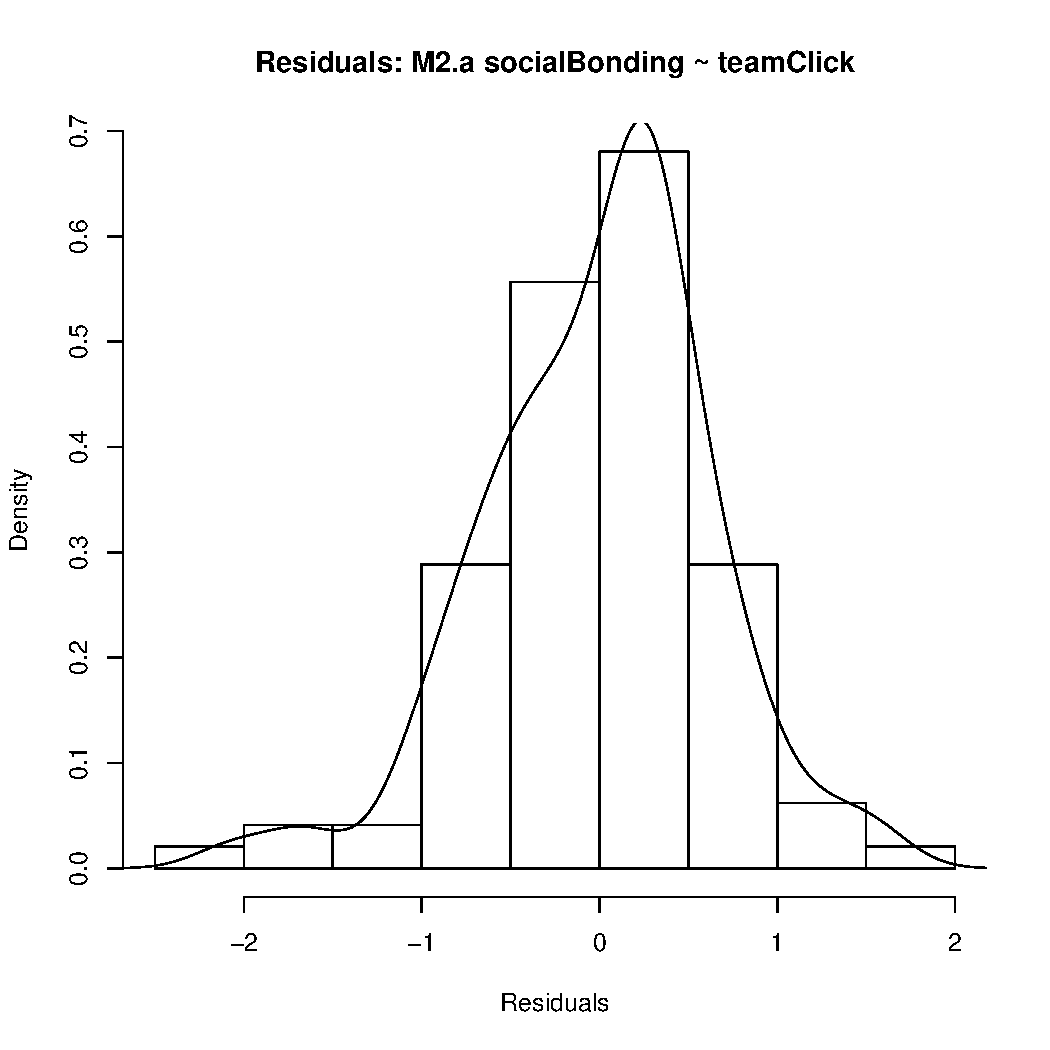
\includegraphics[scale =.4]{images/MLM2aHist.pdf}
  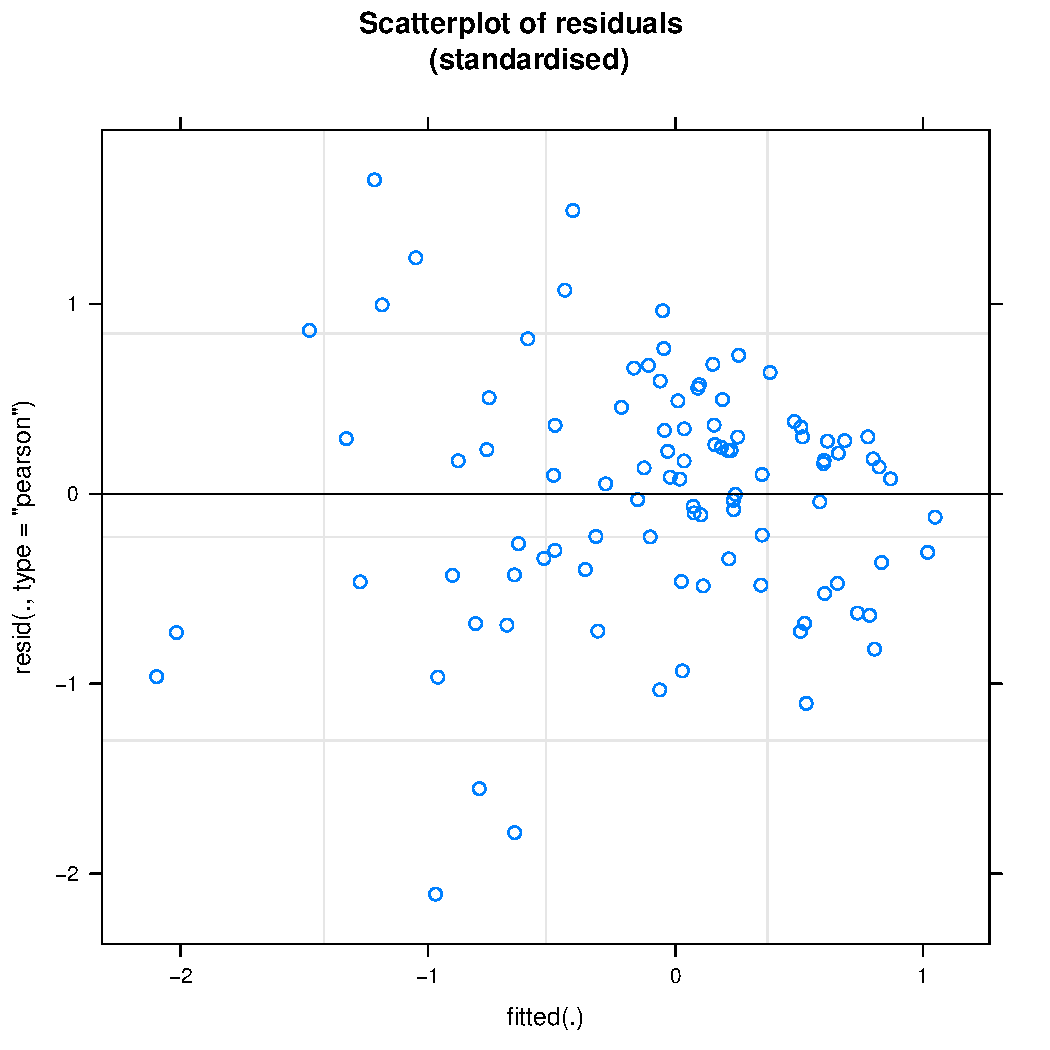
\includegraphics[scale =.4]{images/MLM2aScatter.pdf}
  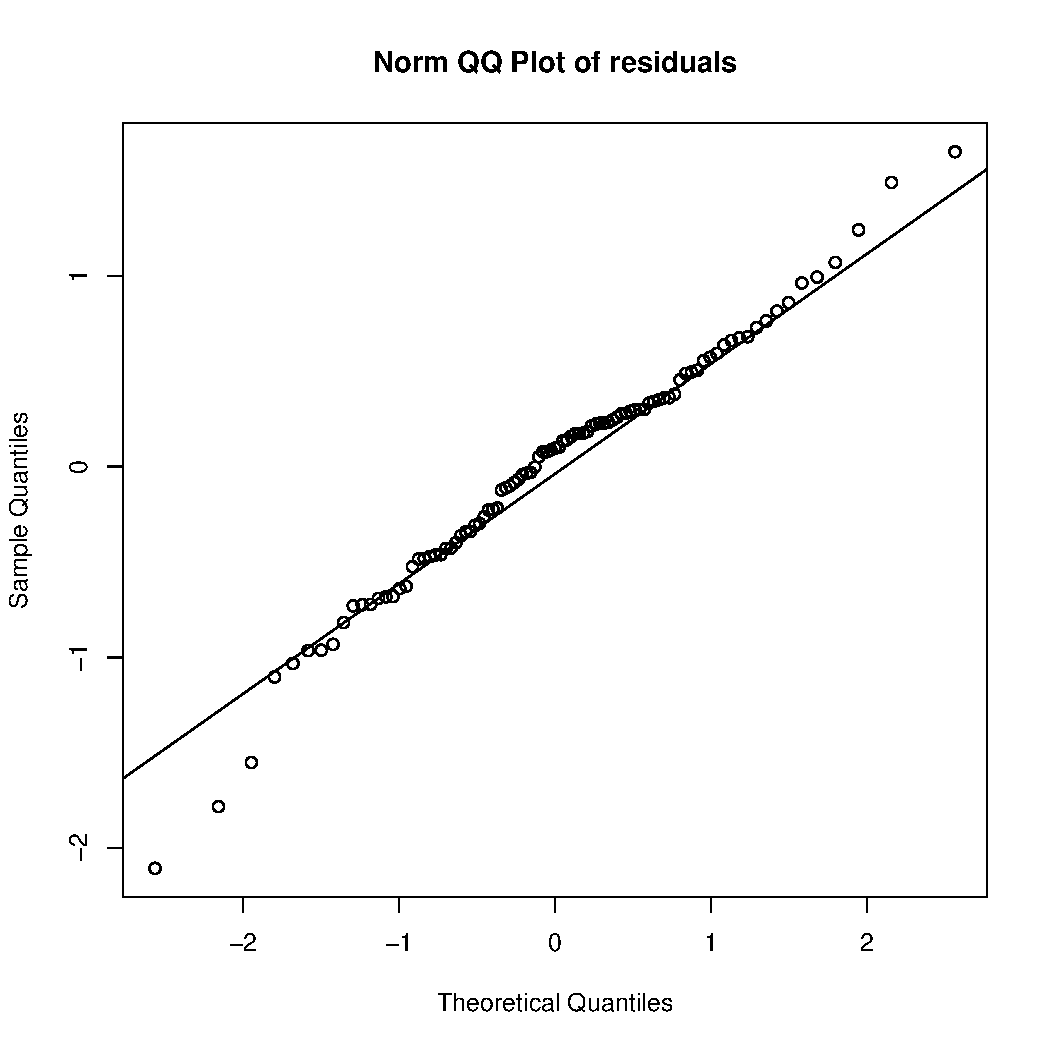
\includegraphics[scale =.4]{images/MLM2aQQNorm.pdf}
  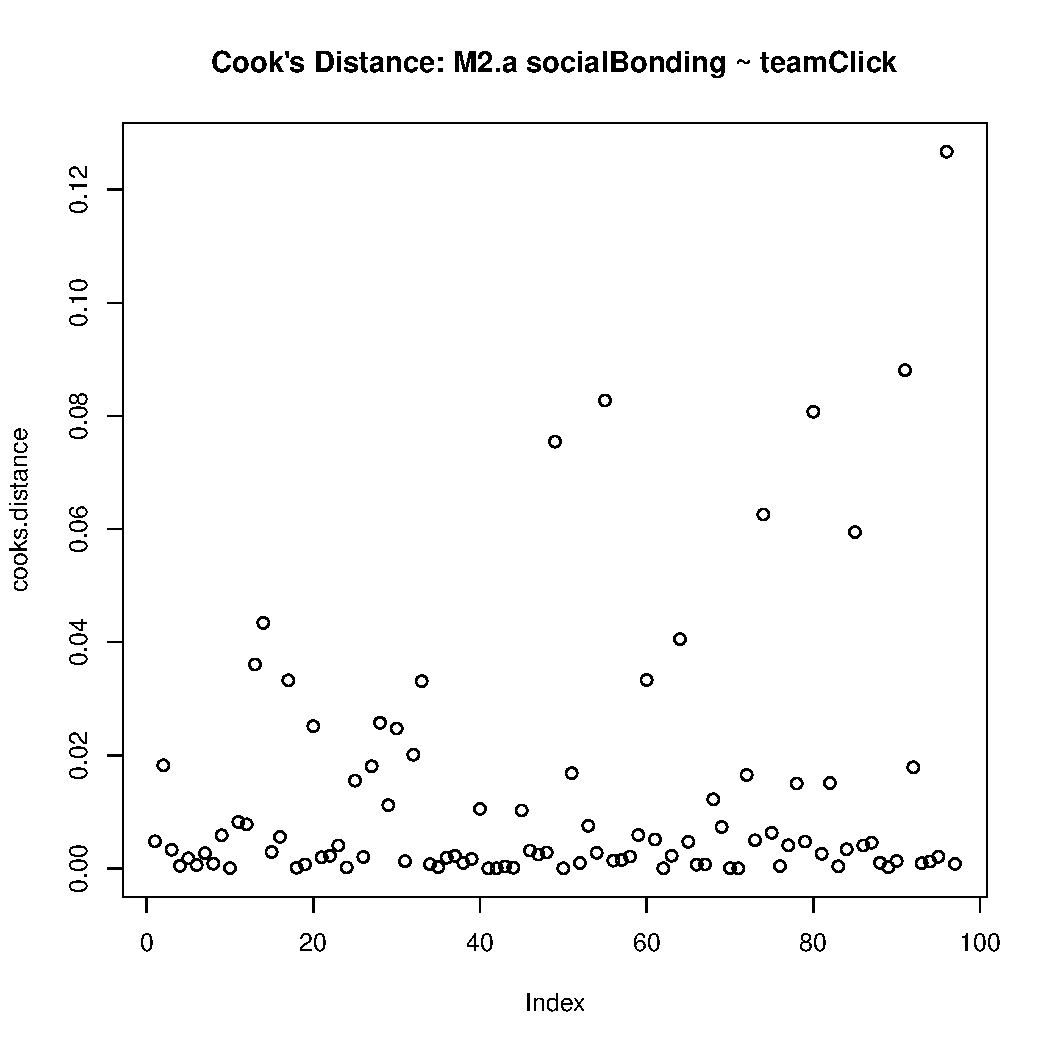
\includegraphics[scale =.4]{images/MLM2aCooksD.pdf}
  \caption{Model Assumptions: M2a Team Click predicts Social Bonding}
  \label{fig:MKM2aAssumptions}
\end{figure}





\begin{figure}[htbp]
  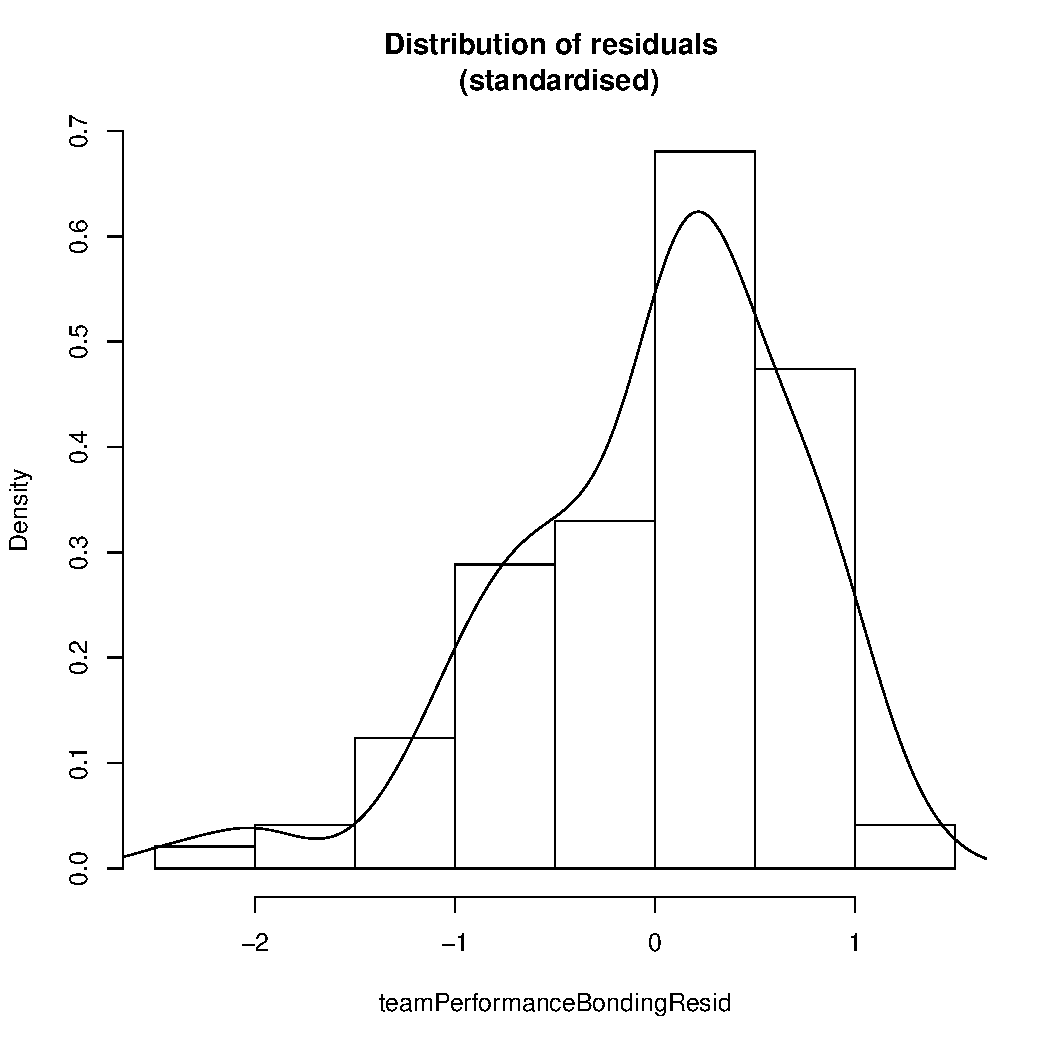
\includegraphics[scale =.4]{images/MLM3aHist.pdf}
  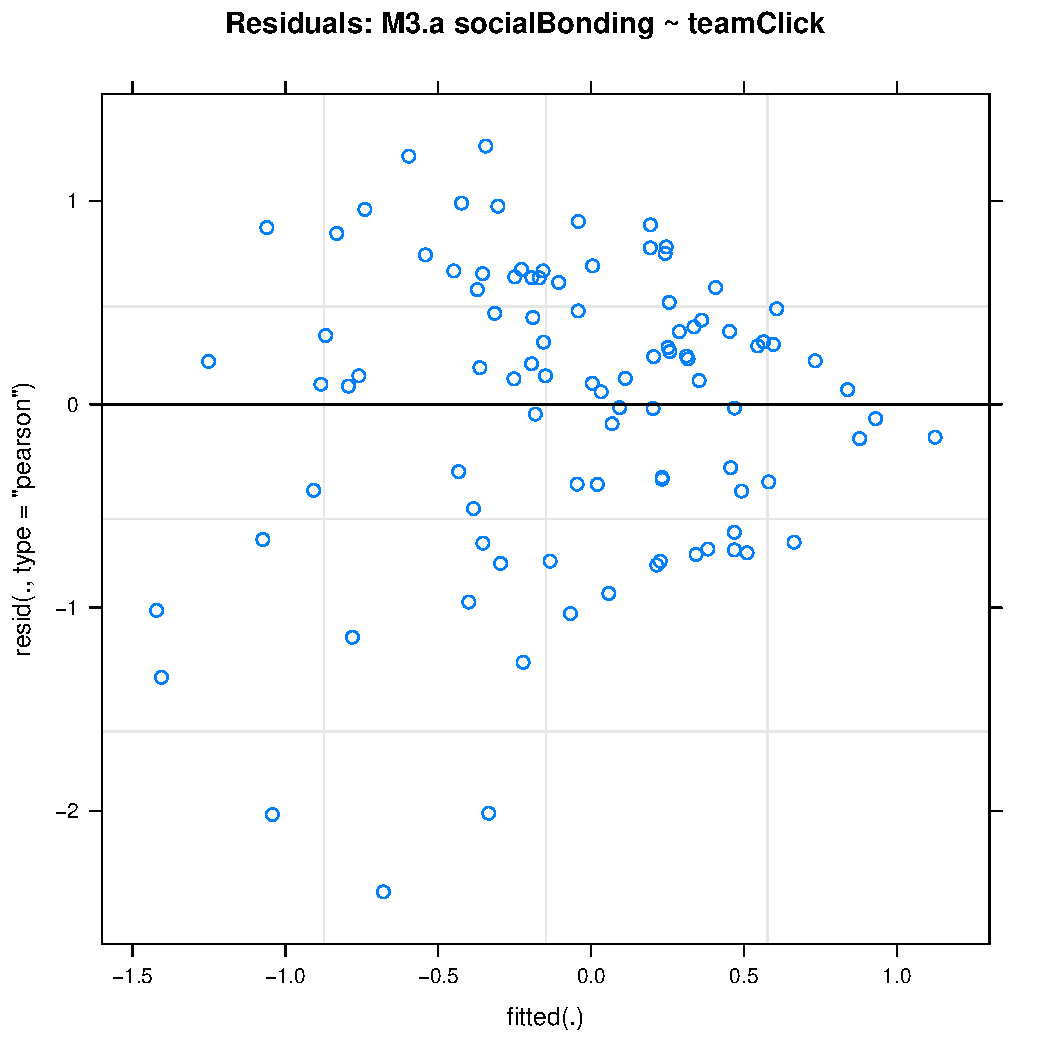
\includegraphics[scale =.4]{images/MLM3aScatter.pdf}
  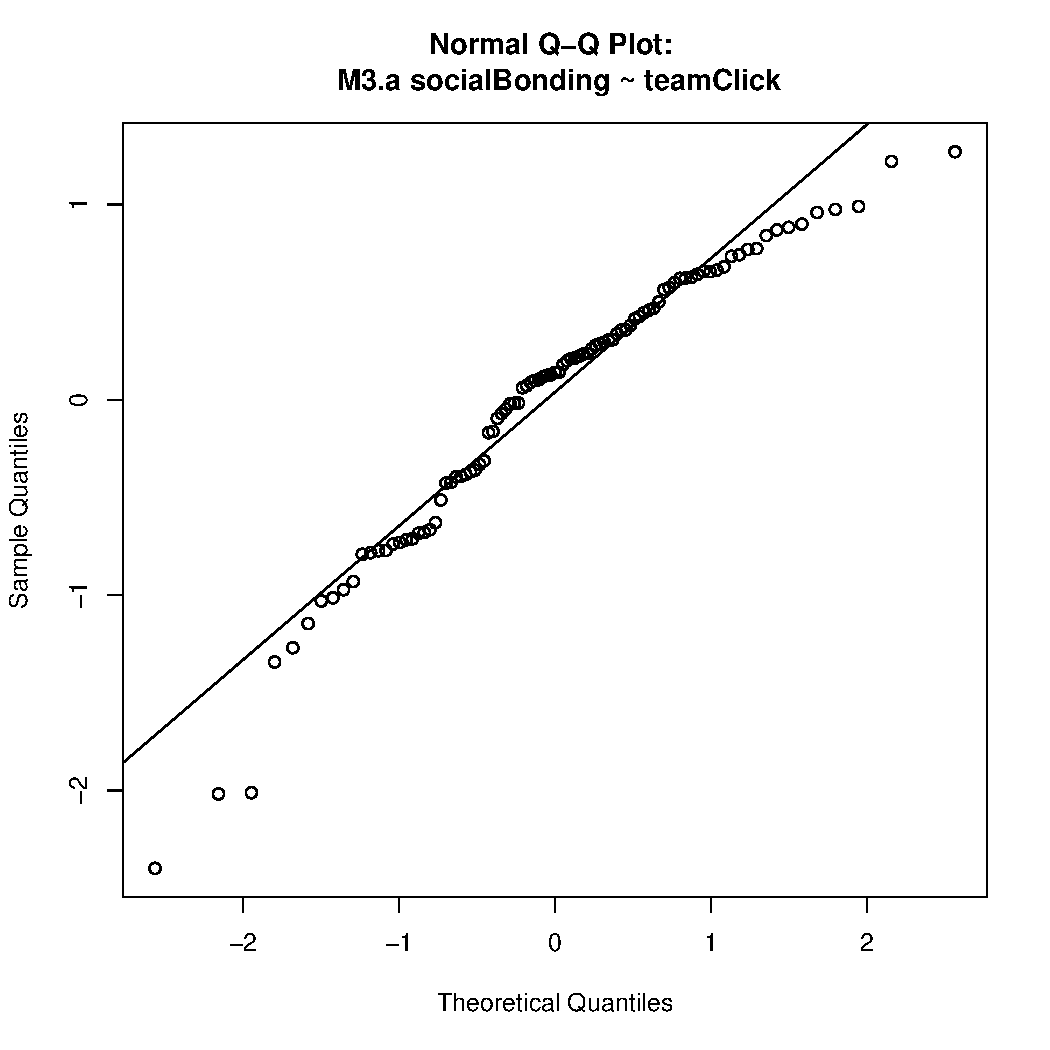
\includegraphics[scale =.4]{images/MLM3aQQNorm.pdf}
  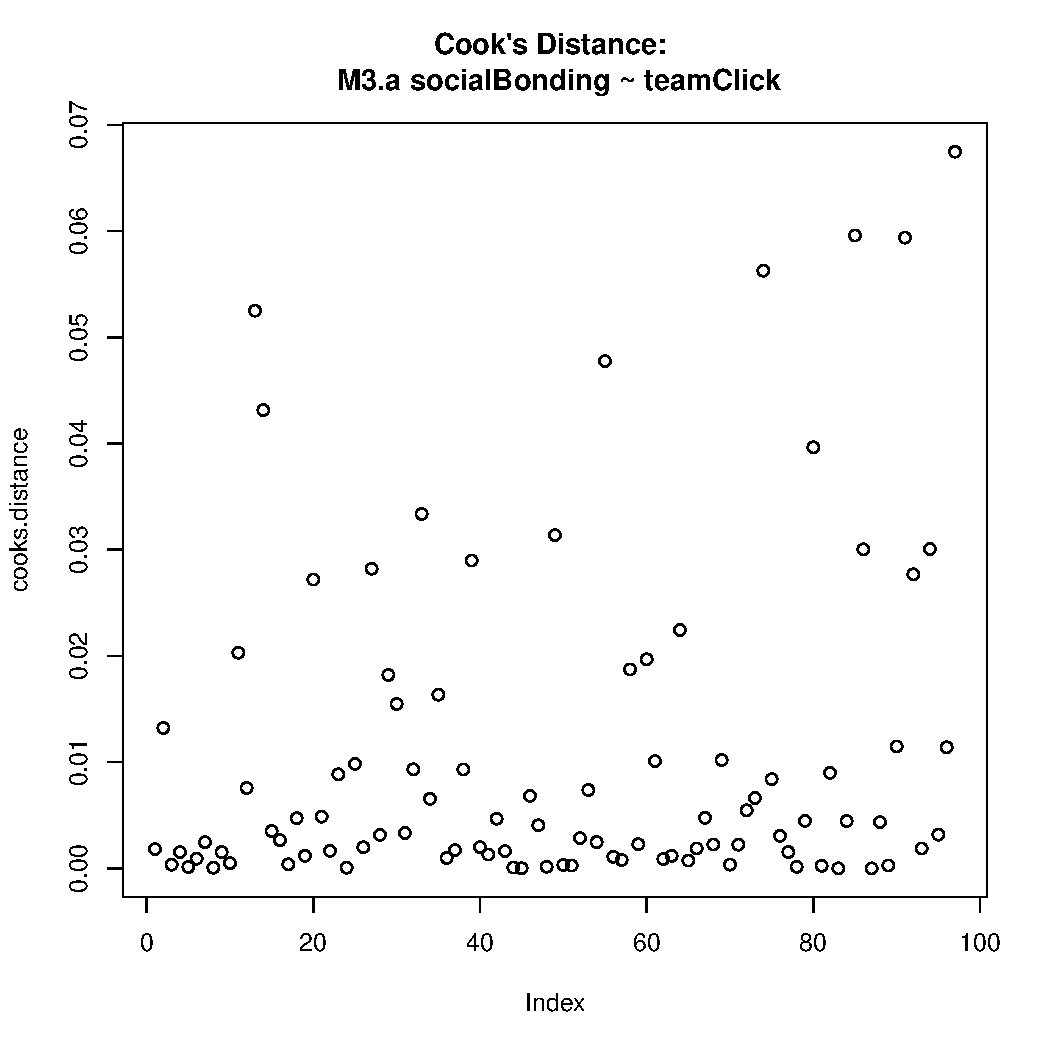
\includegraphics[scale =.4]{images/MLM3aCooksD.pdf}
  \caption{Model Assumptions: M3a Joint Action Success predicts Social Bonding}
  \label{fig:MLM3aAssumptions}
\end{figure}

\begin{figure}[htbp]
  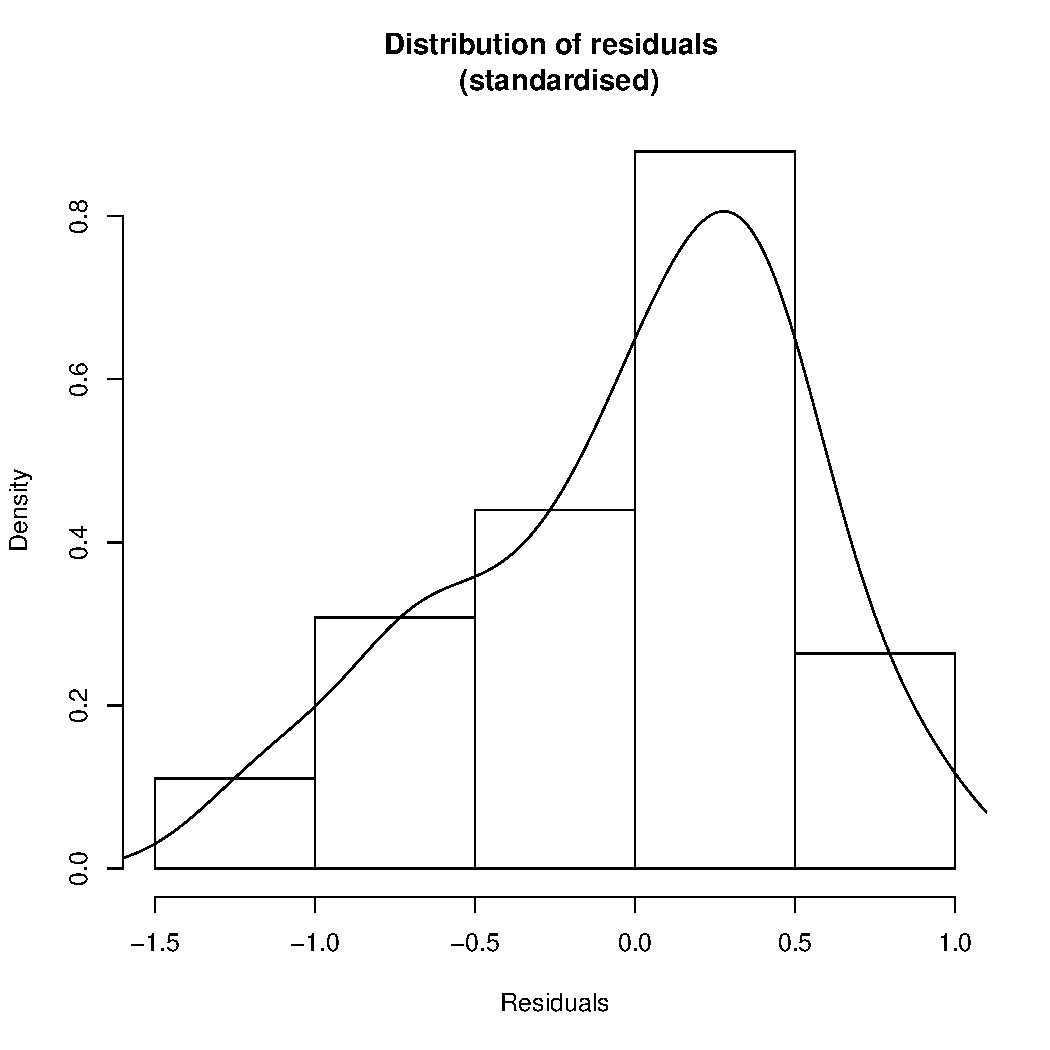
\includegraphics[scale =.4]{images/MLM3aOutHist.pdf}
  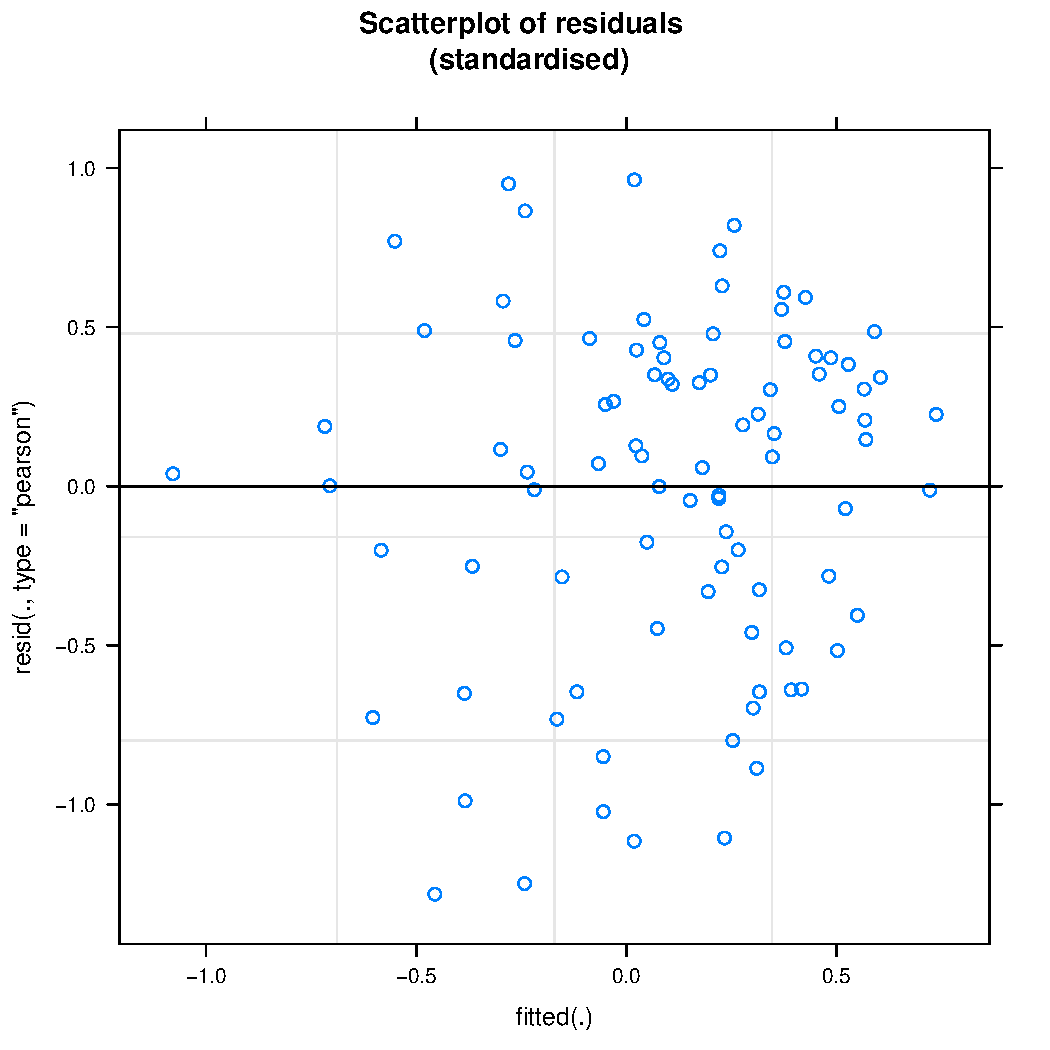
\includegraphics[scale =.4]{images/MLM3aOutScatter.pdf}
  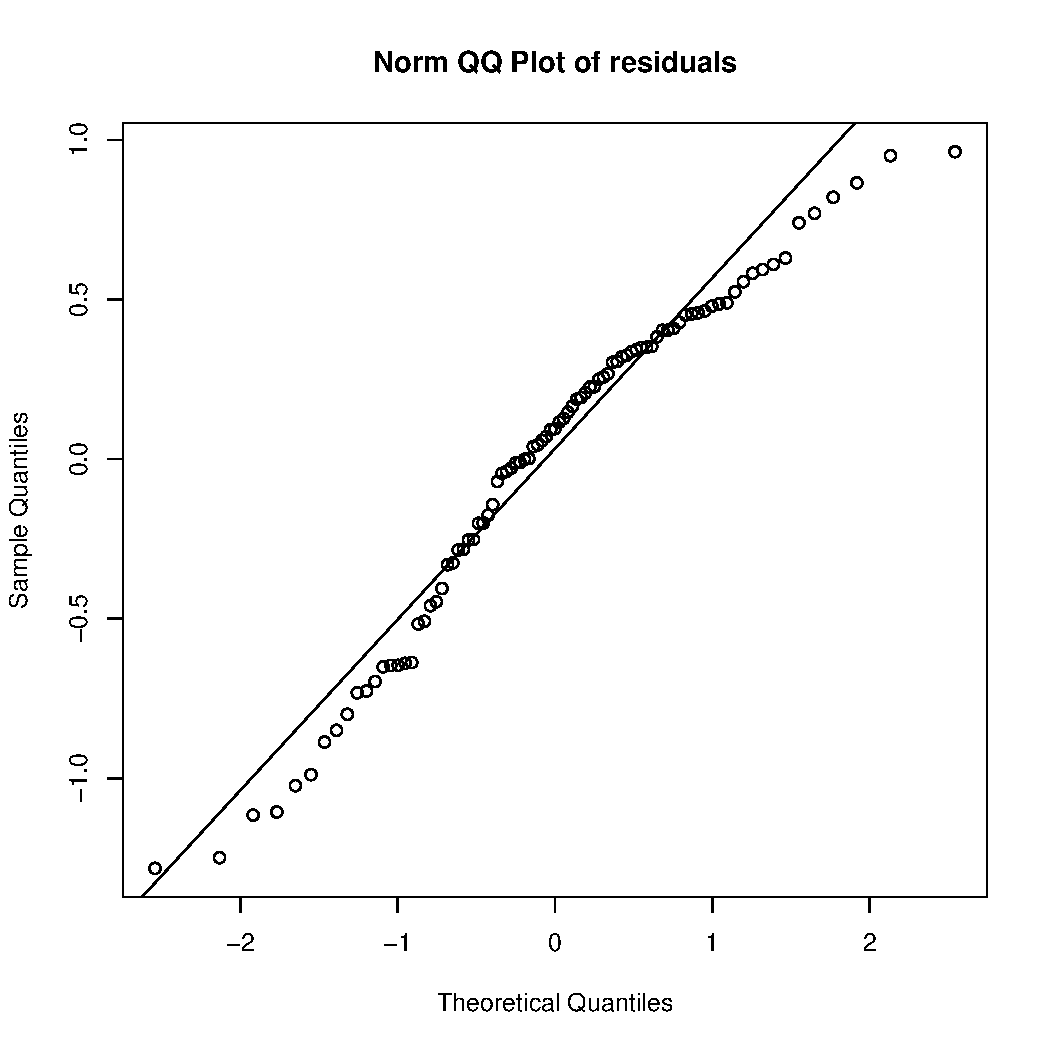
\includegraphics[scale =.4]{images/MLM3aOutQQNorm.pdf}
  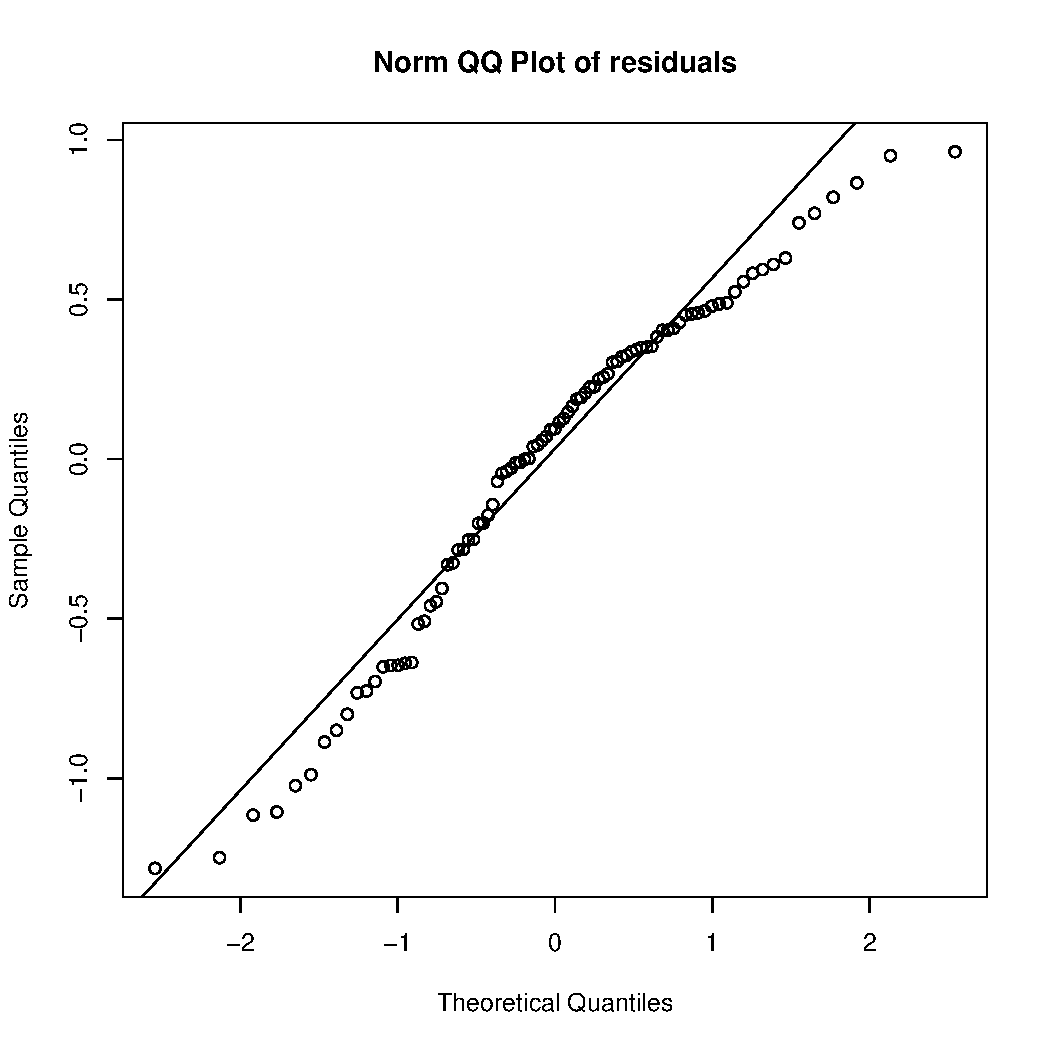
\includegraphics[scale =.4]{images/MLM3aOutCooksD.pdf}
  \caption{Model Assumptions: M3a Joint Action Success predicts Social Bonding (outliers removed)}
  \label{fig:MLM3aOutAssumptions}
\end{figure}

\begin{figure}[htbp]
  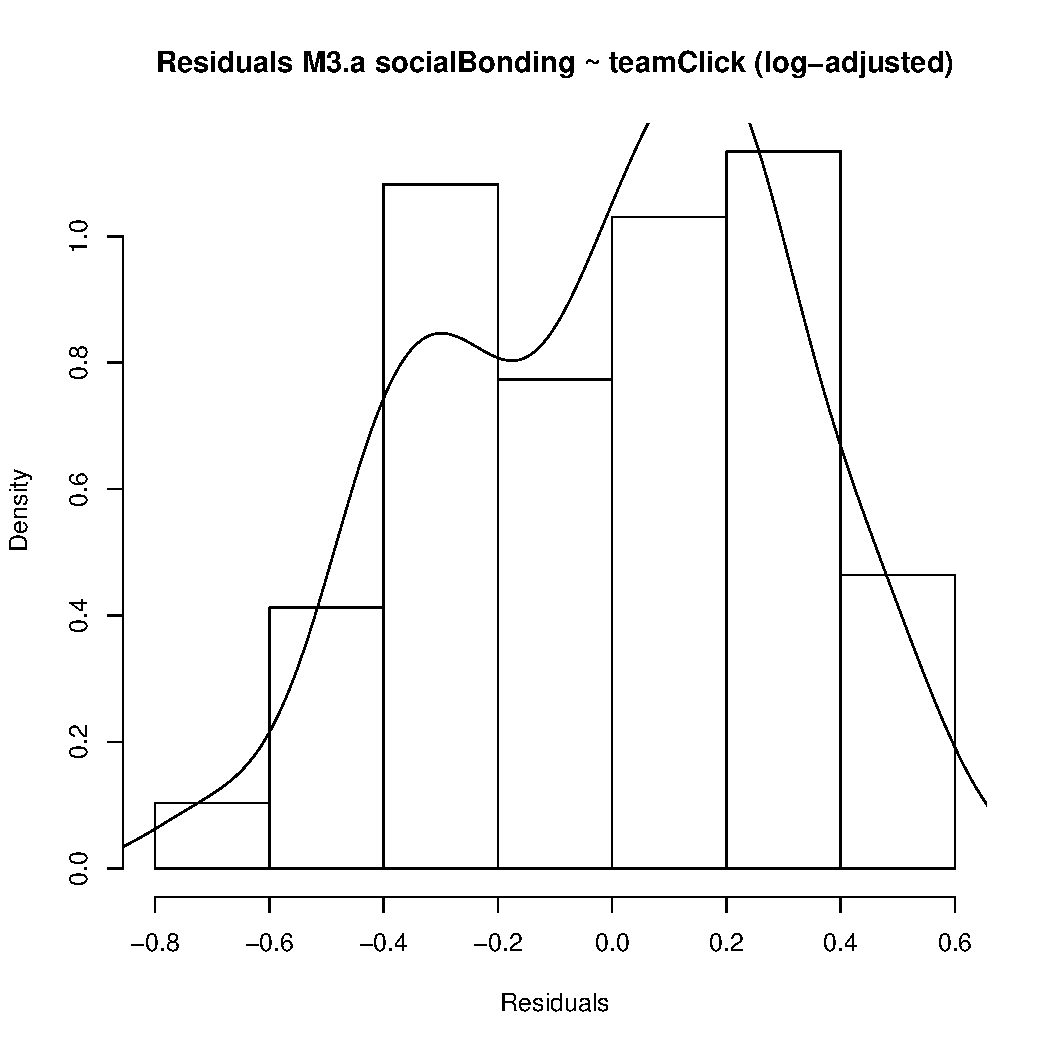
\includegraphics[scale =.4]{images/MLM3aLogHist.pdf}
  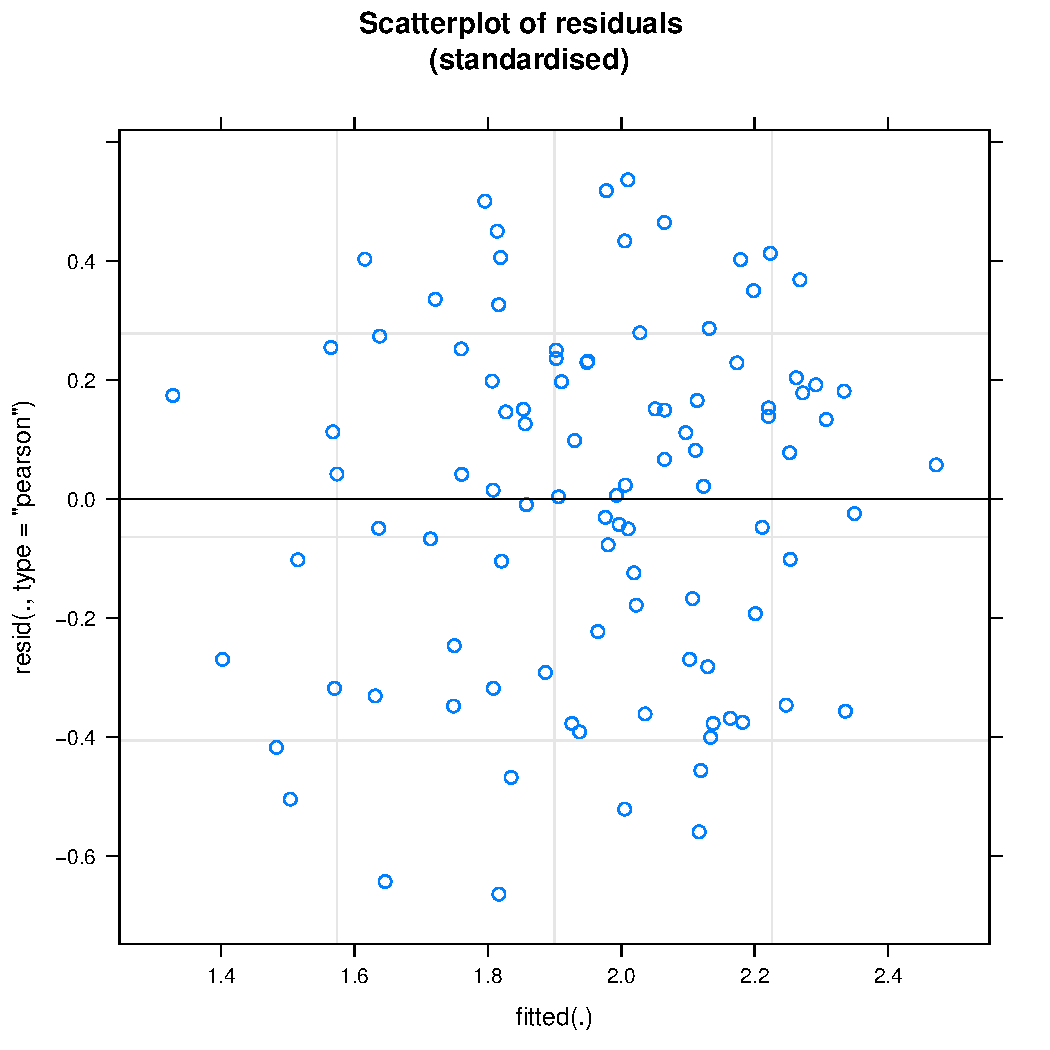
\includegraphics[scale =.4]{images/MLM3aLogScatter.pdf}
  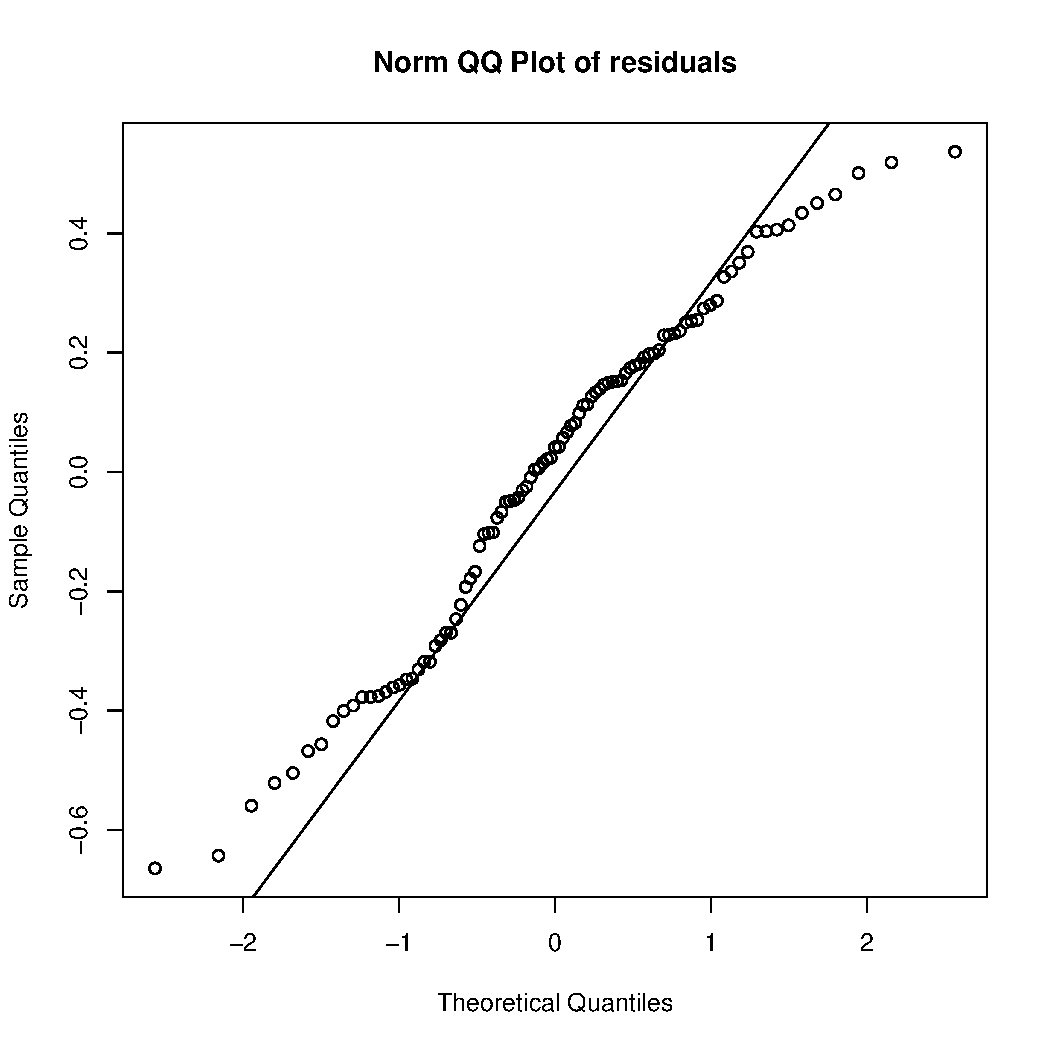
\includegraphics[scale =.4]{images/MLM3aLogQQNorm.pdf}
  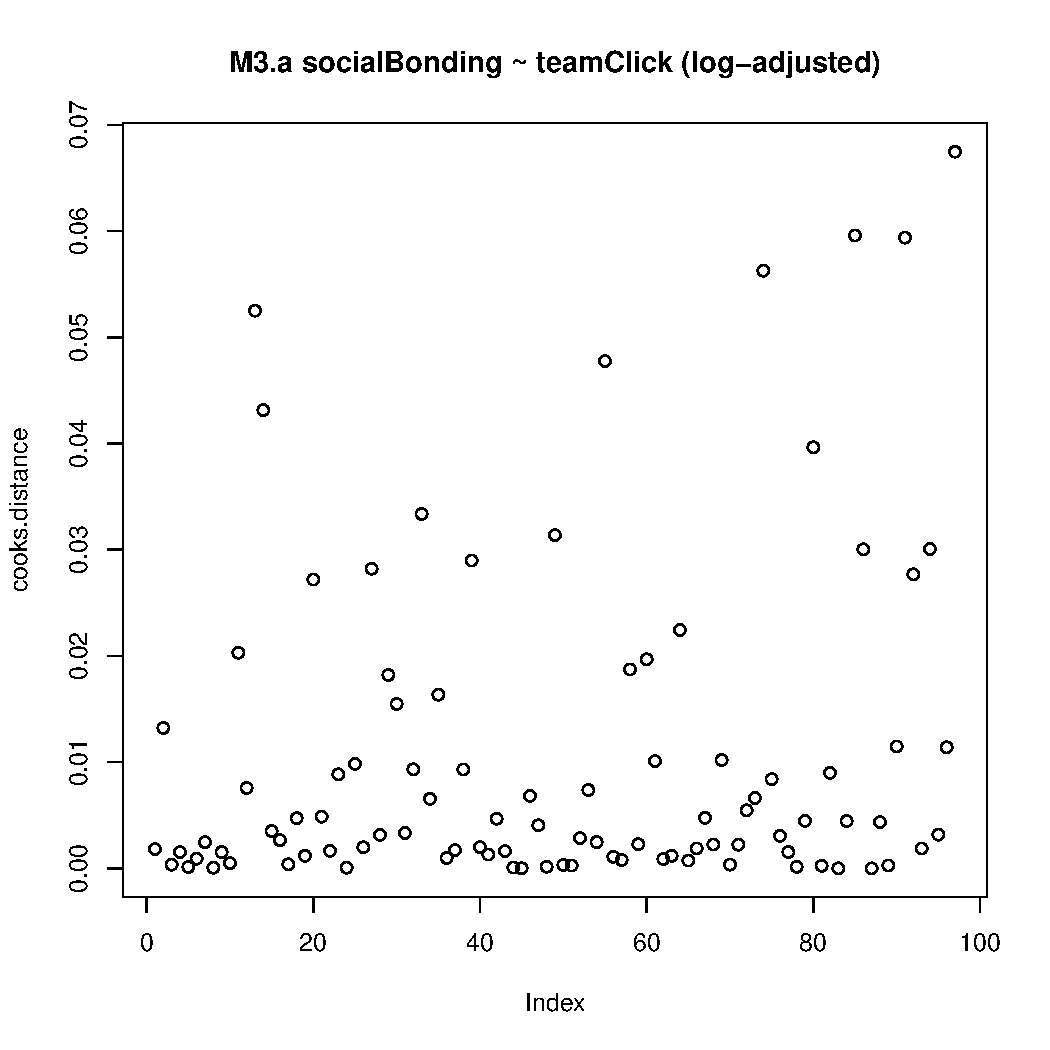
\includegraphics[scale =.4]{images/MLM3aLogCooksD.pdf}
  \caption{Model Assumptions: M3a Joint Action Success predicts Social Bonding (log-transformed)}
  \label{fig:MLM3aLogAssumptions}
\end{figure}








\begin{figure}[htbp]
  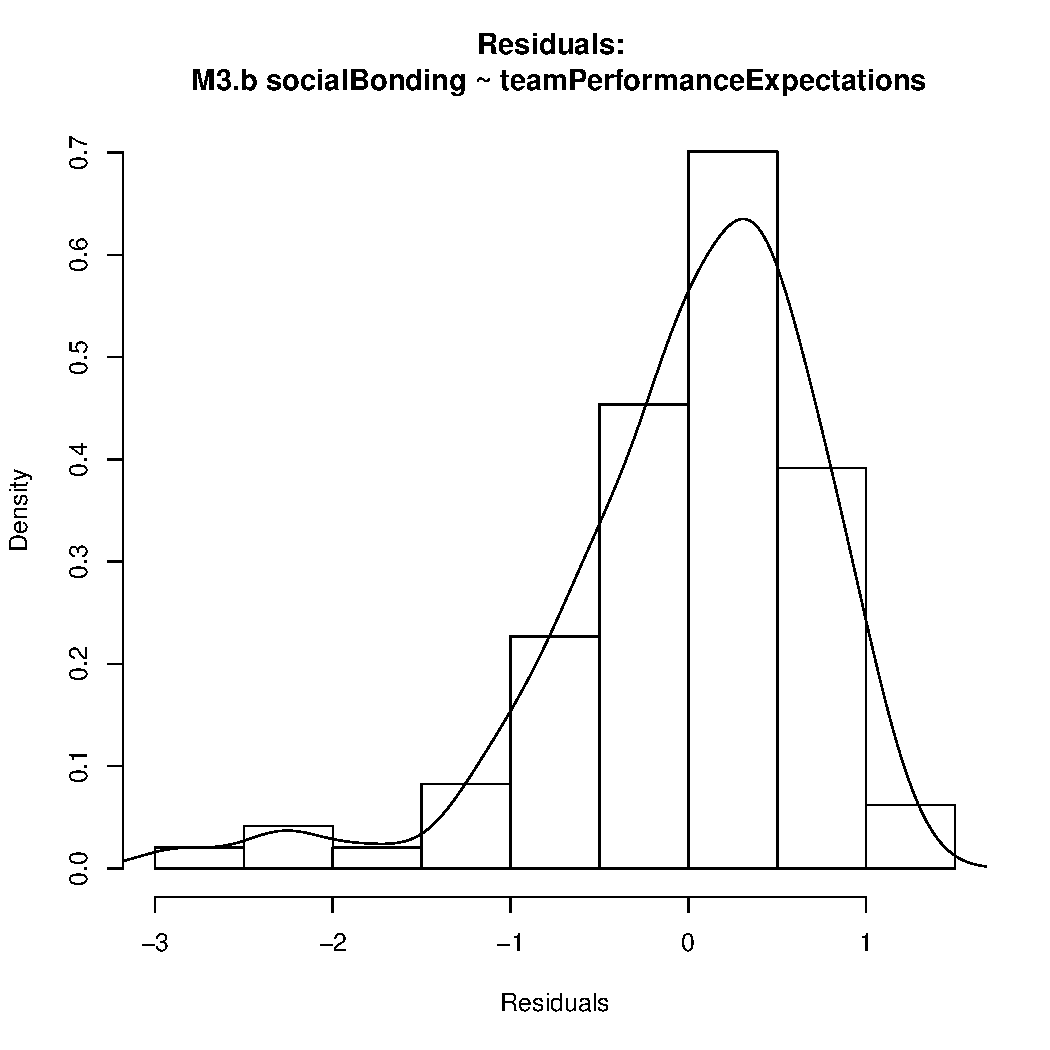
\includegraphics[scale =.4]{images/MLM3bHist.pdf}
  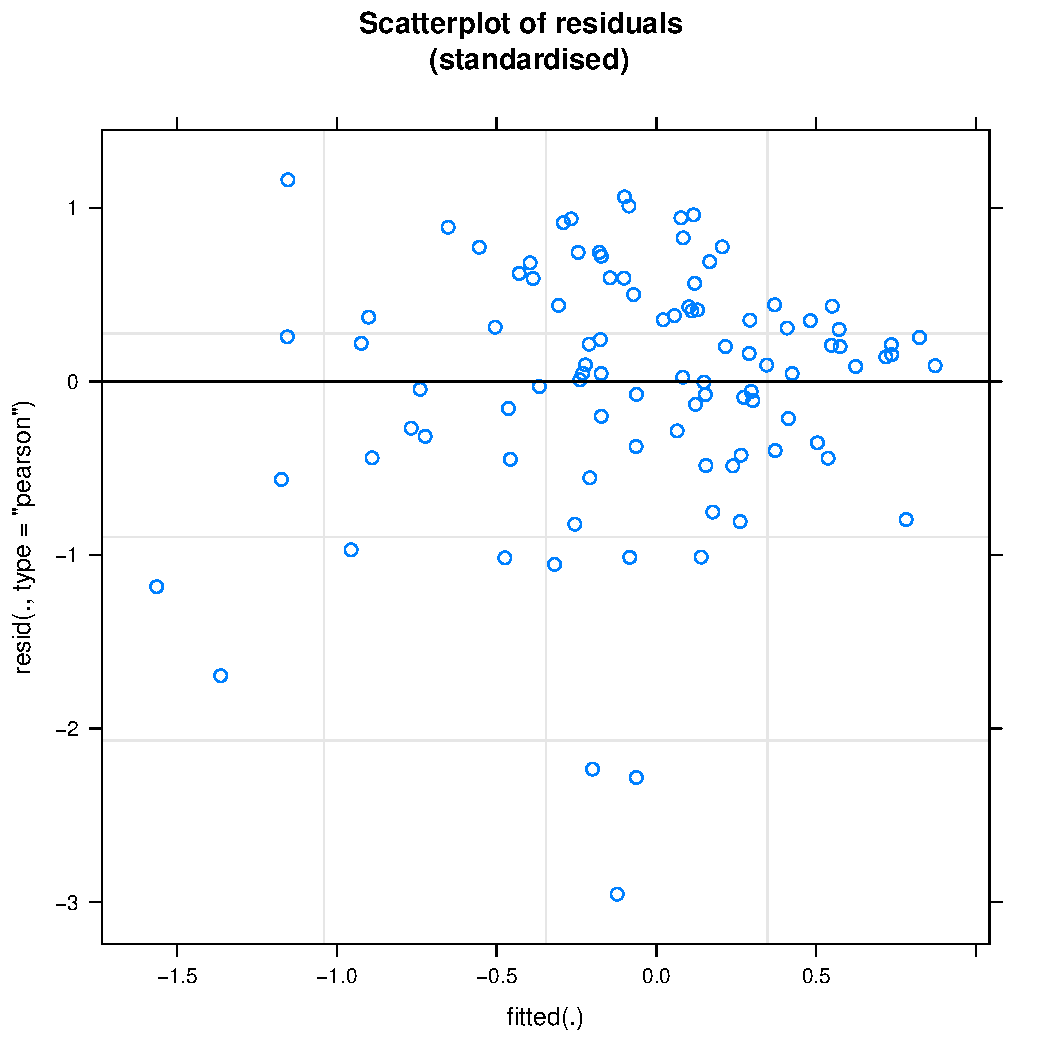
\includegraphics[scale =.4]{images/MLM3bScatter.pdf}
  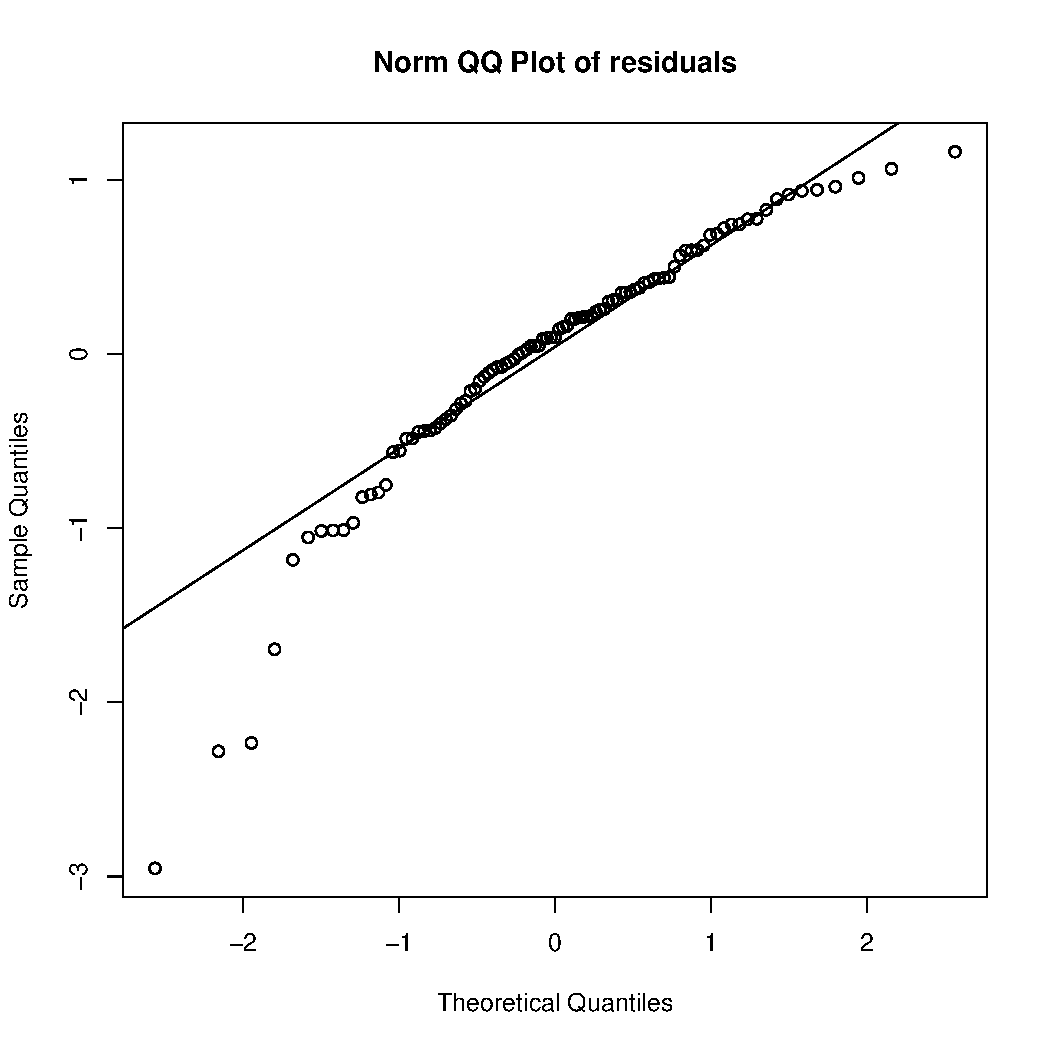
\includegraphics[scale =.4]{images/MLM3bQQNorm.pdf}
  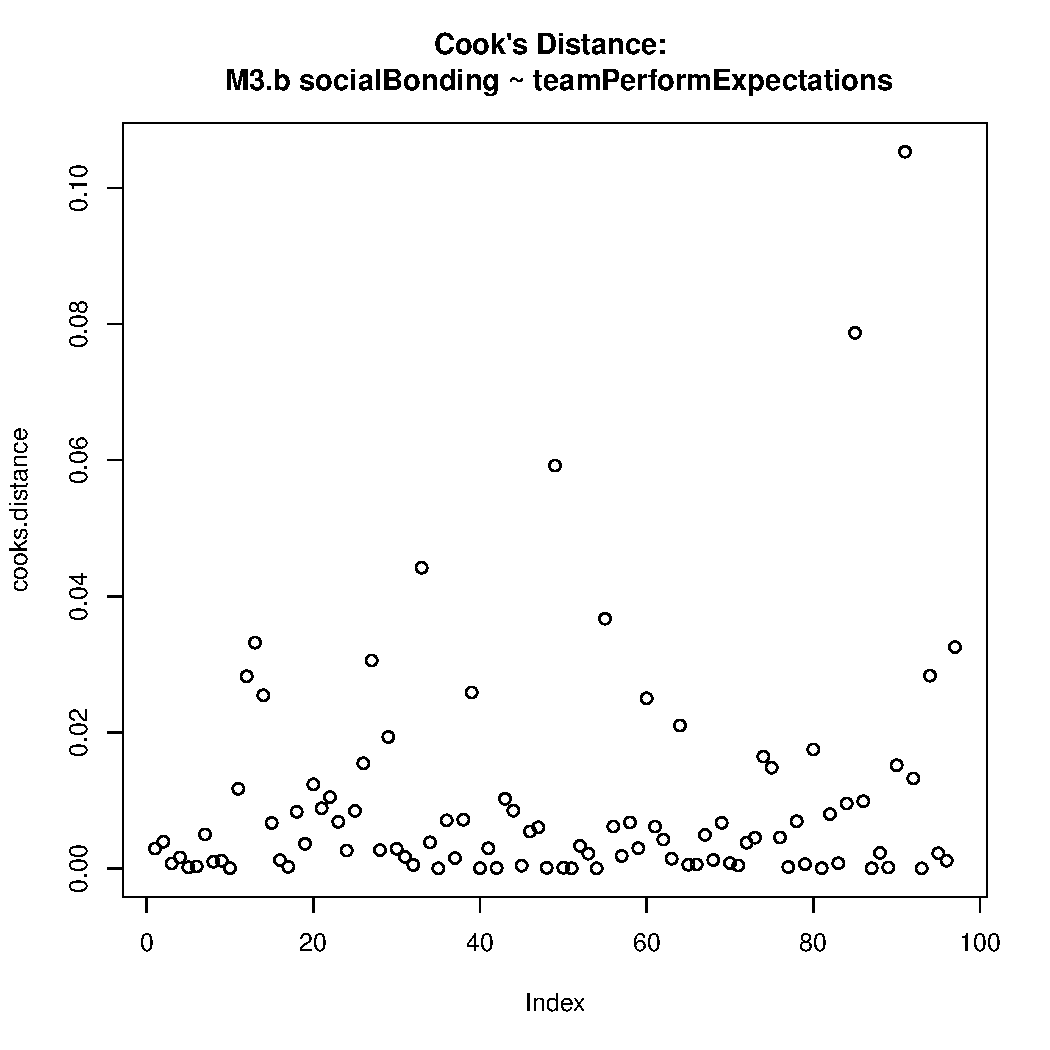
\includegraphics[scale =.4]{images/MLM3bCooksD.pdf}
  \caption{Model Assumptions: M3a Joint Action Success predicts Social Bonding (log-transformed)}
  \label{fig:MLM3bAssumptions}
\end{figure}

\begin{figure}[htbp]
  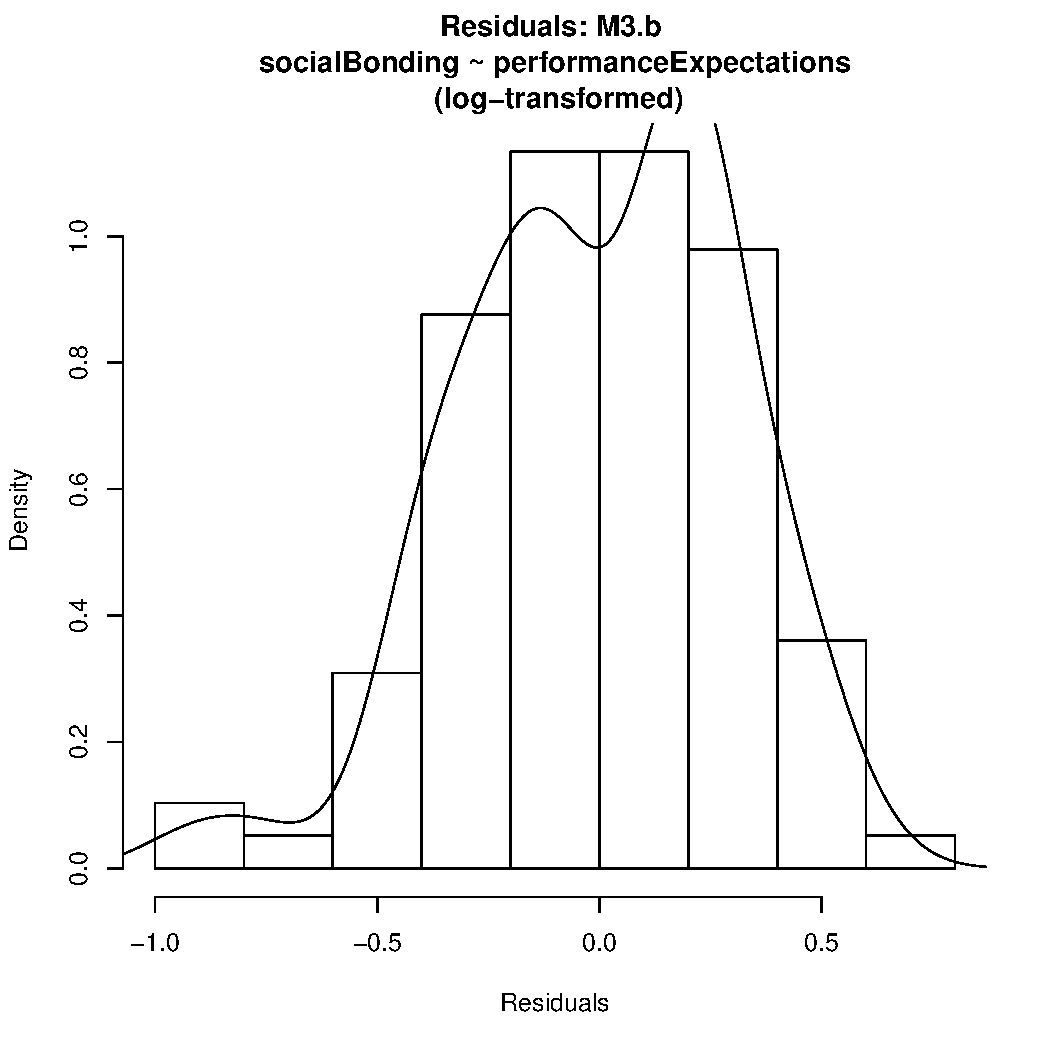
\includegraphics[scale =.4]{images/MLM3bLogHist.pdf}
  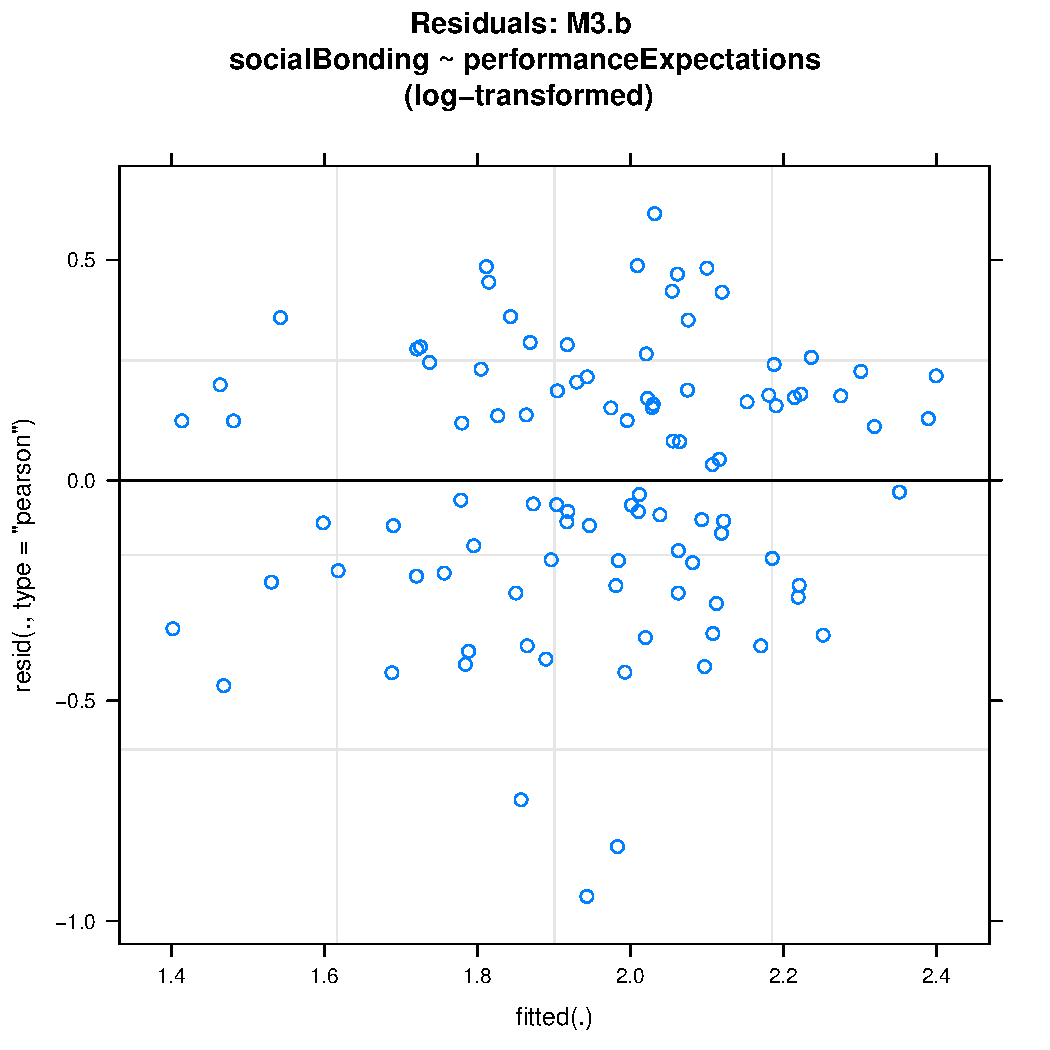
\includegraphics[scale =.4]{images/MLM3bLogScatter.pdf}
  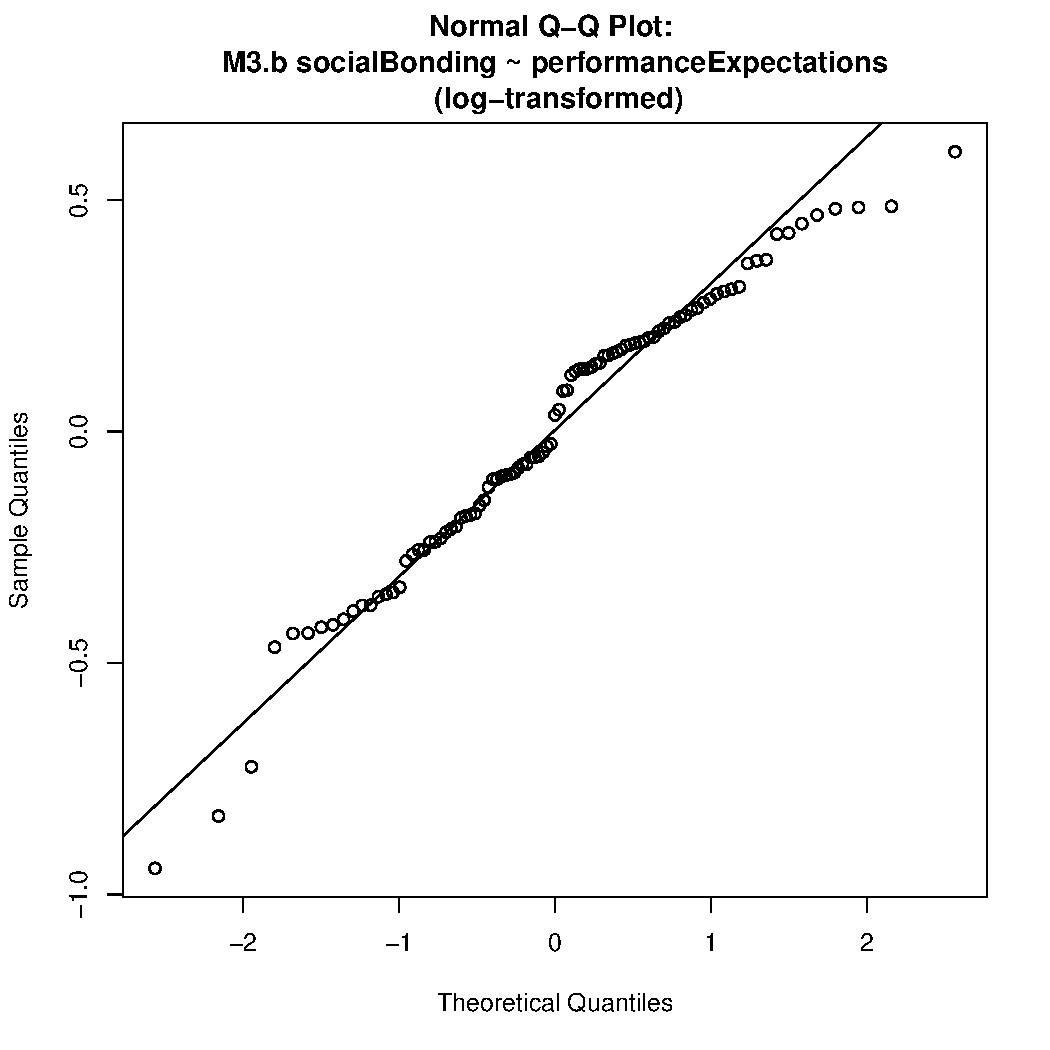
\includegraphics[scale =.4]{images/MLM3bLogQQNorm.pdf}
  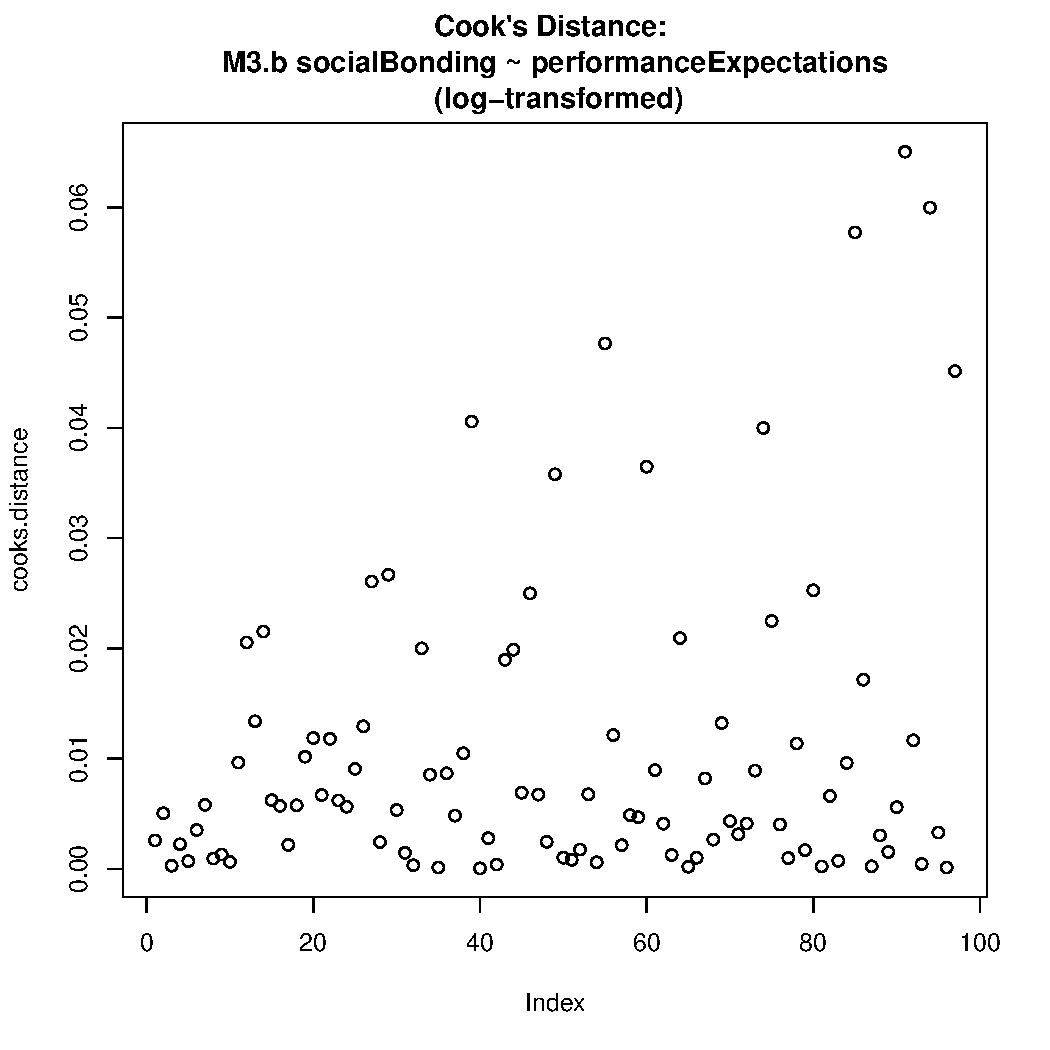
\includegraphics[scale =.4]{images/MLM3bLogCooksD.pdf}
  \caption{Model Assumptions: M3a Joint Action Success predicts Social Bonding (log-transformed)}
  \label{fig:MLM3bLogAssumptions}
\end{figure}






\begin{figure}[htbp]
  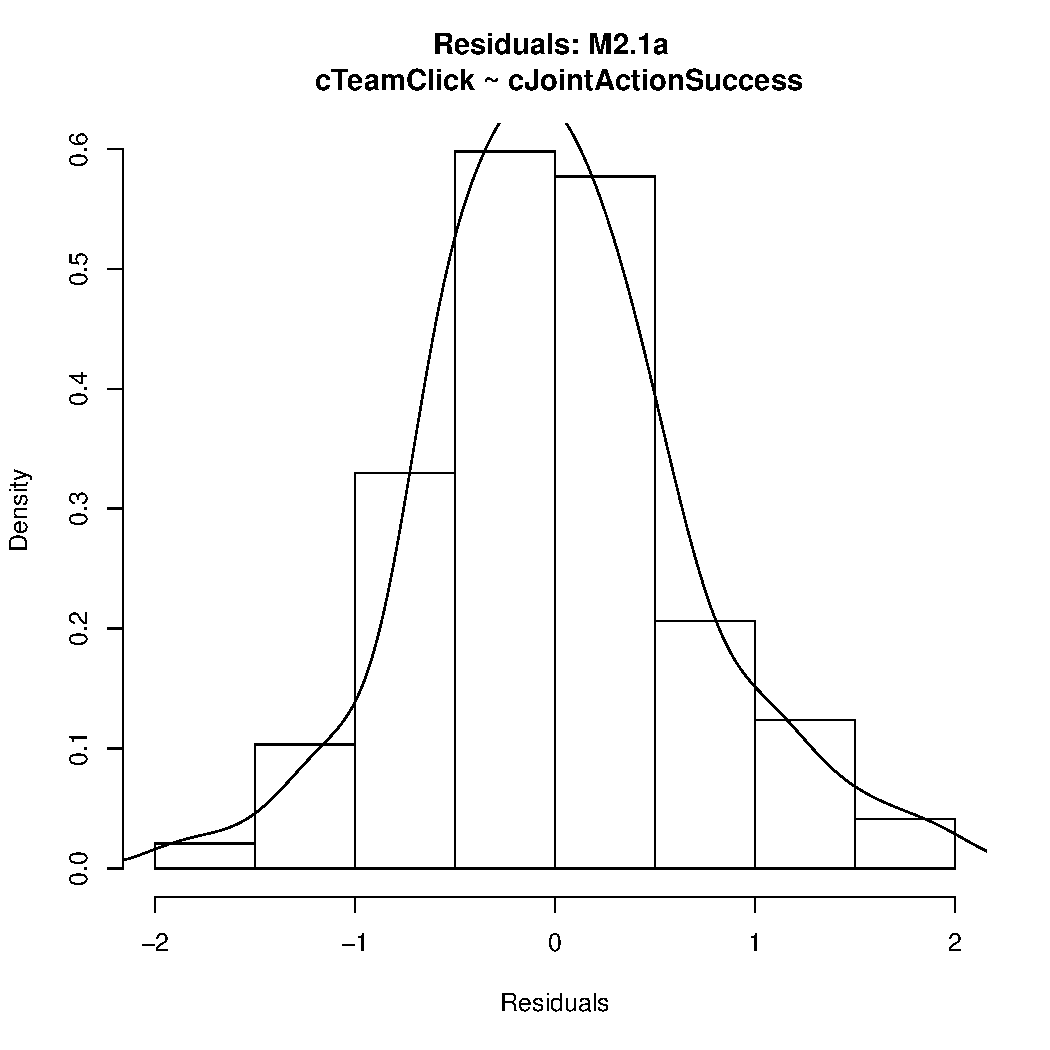
\includegraphics[scale =.4]{images/MLM21aHist.pdf}
  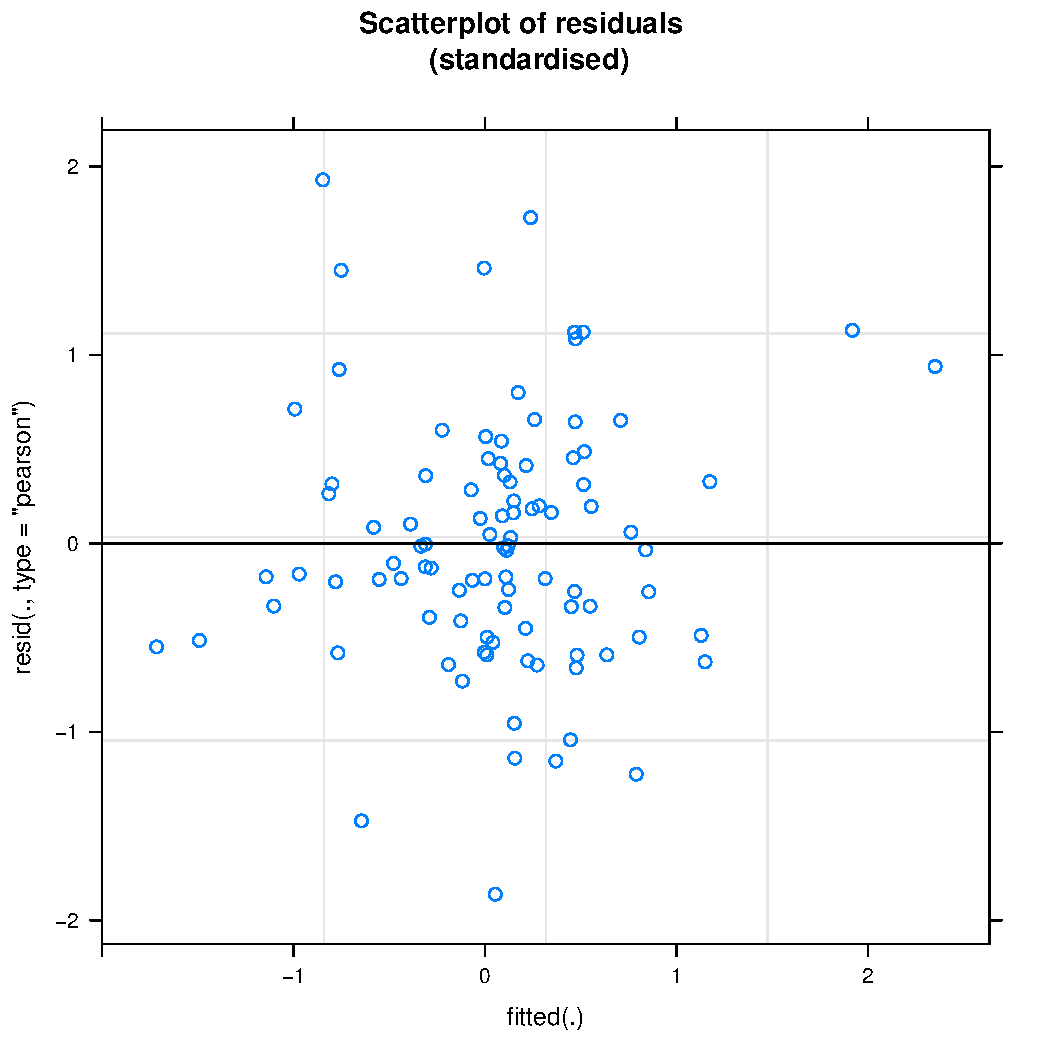
\includegraphics[scale =.4]{images/MLM21aScatter.pdf}
  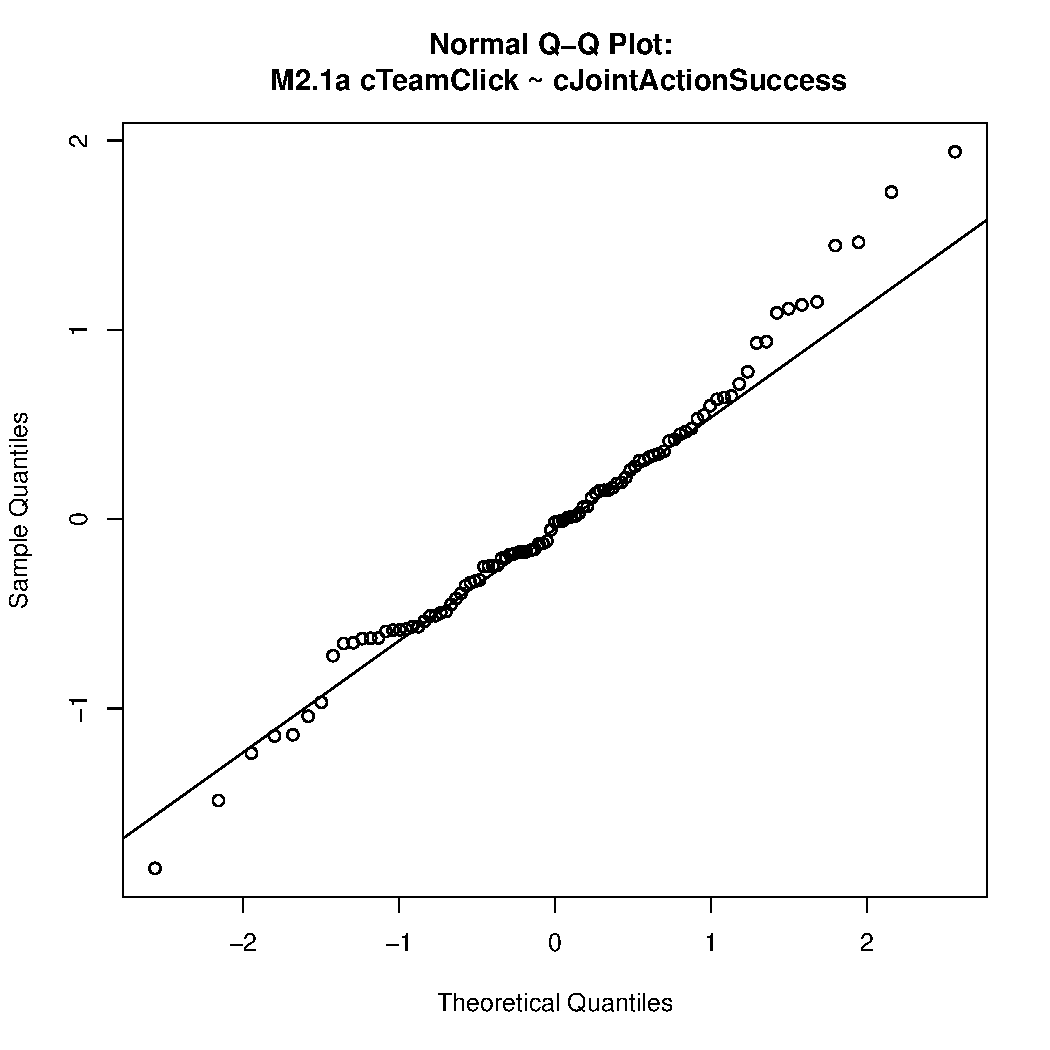
\includegraphics[scale =.4]{images/MLM21aQQNorm.pdf}
  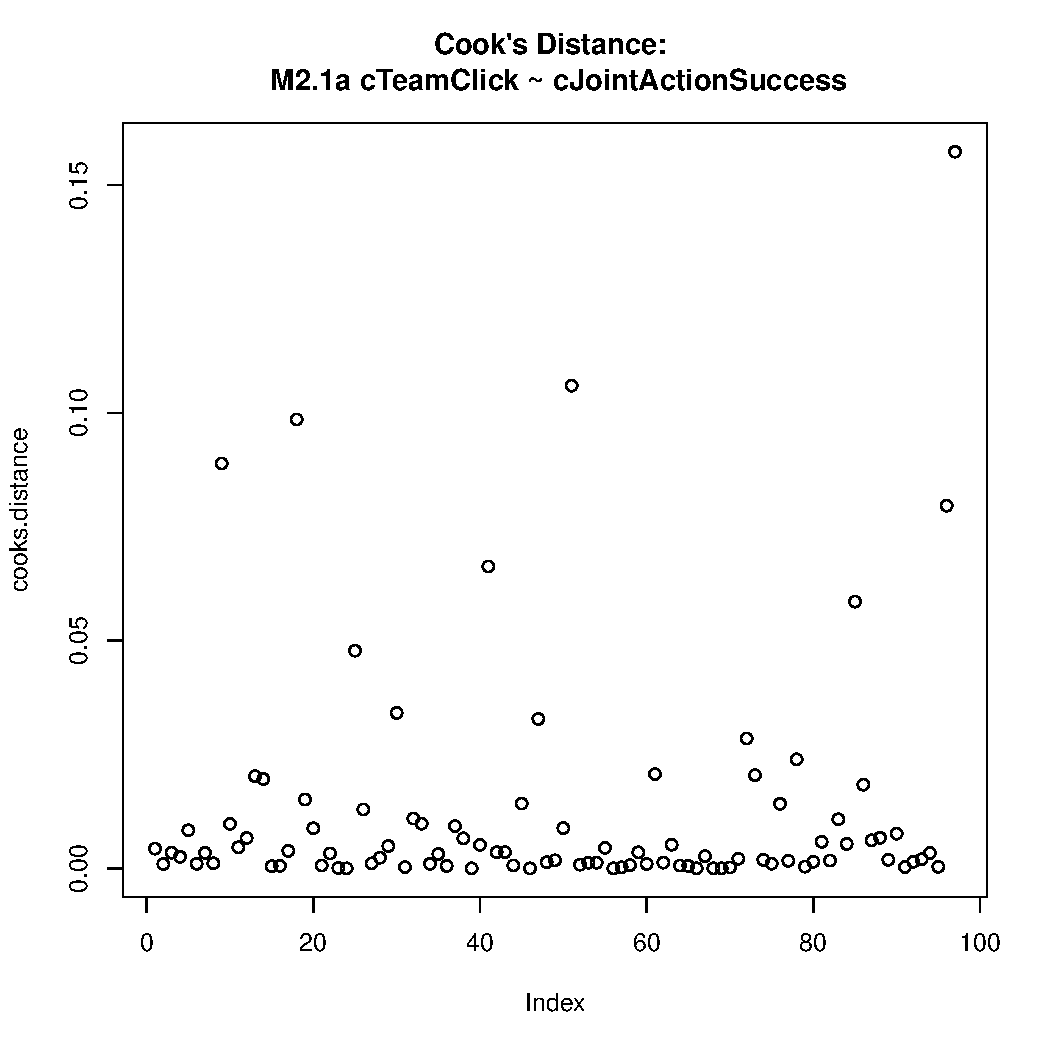
\includegraphics[scale =.4]{images/MLM21aCooksD.pdf}
  \caption{Model Assumptions: M2.1a Change in Joint Action Success predicts change in Team Click}
  \label{fig:MLM21aAssumptions}
\end{figure}





\begin{figure}[htbp]
  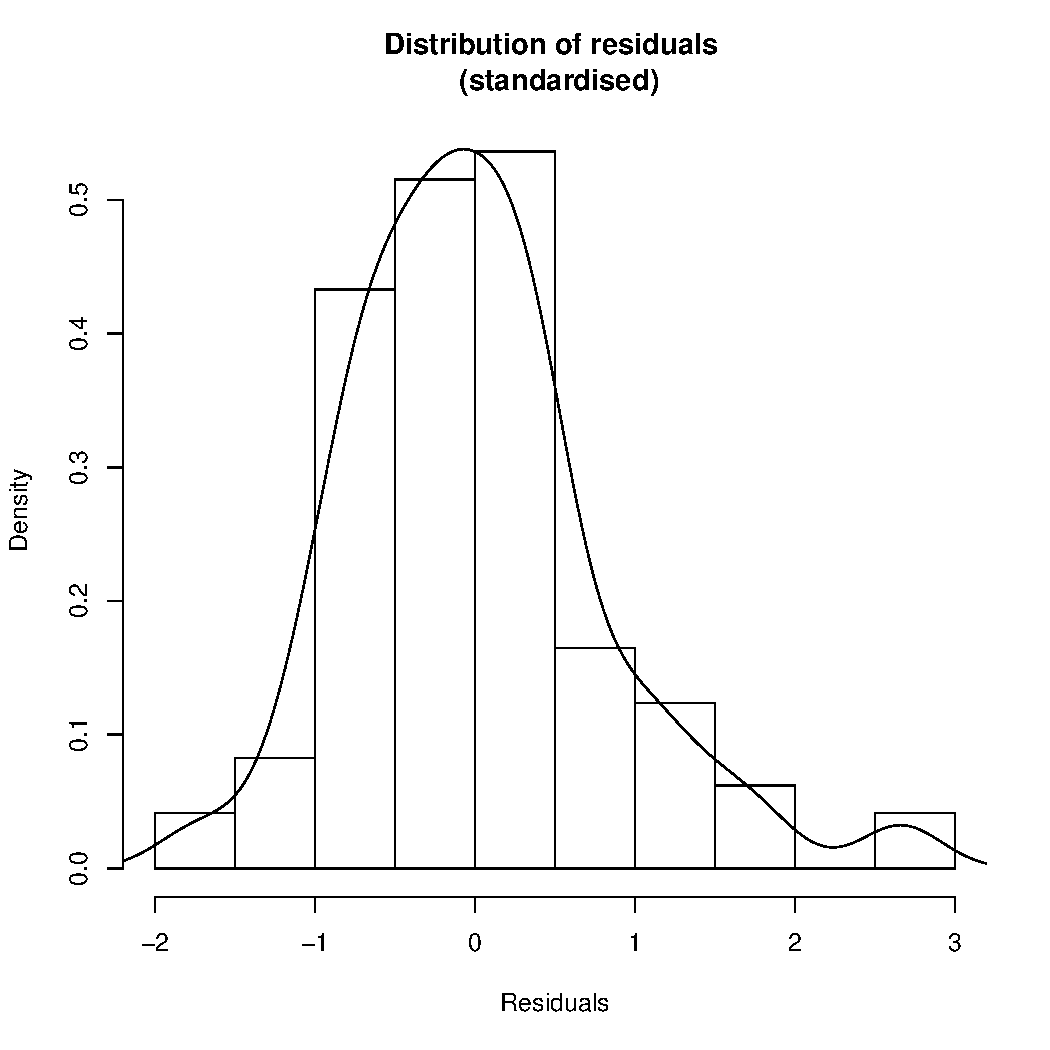
\includegraphics[scale =.4]{images/MLM21bHist.pdf}
  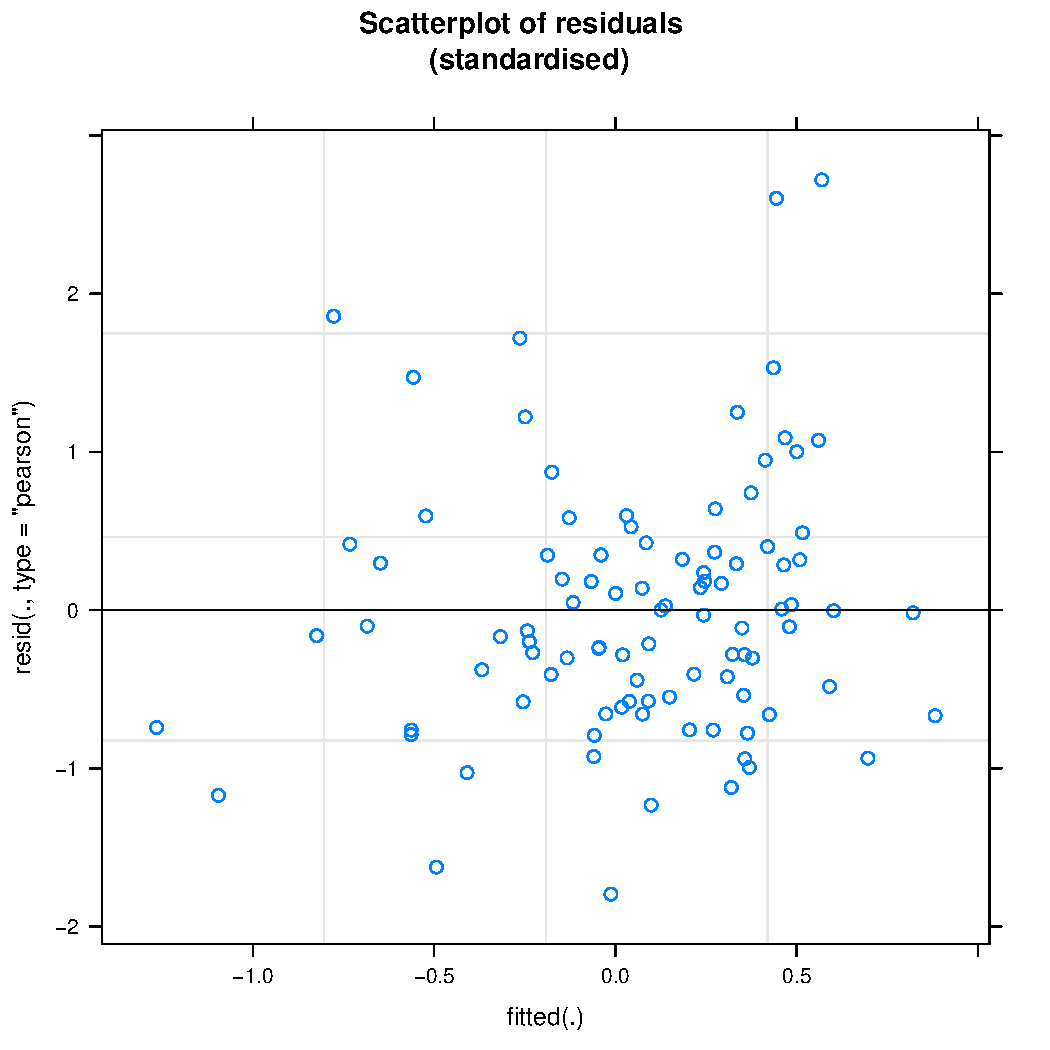
\includegraphics[scale =.4]{images/MLM21bScatter.pdf}
  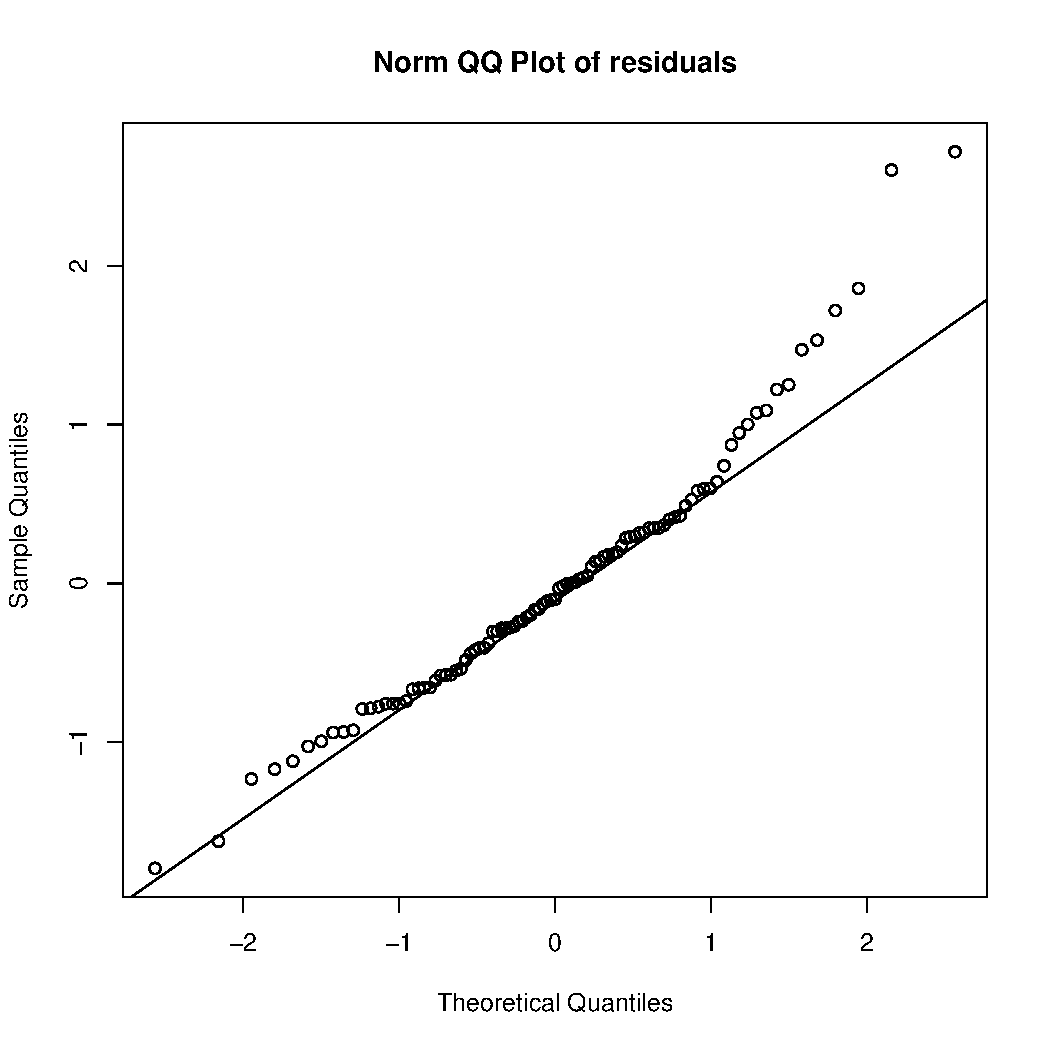
\includegraphics[scale =.4]{images/MLM21bQQNorm.pdf}
  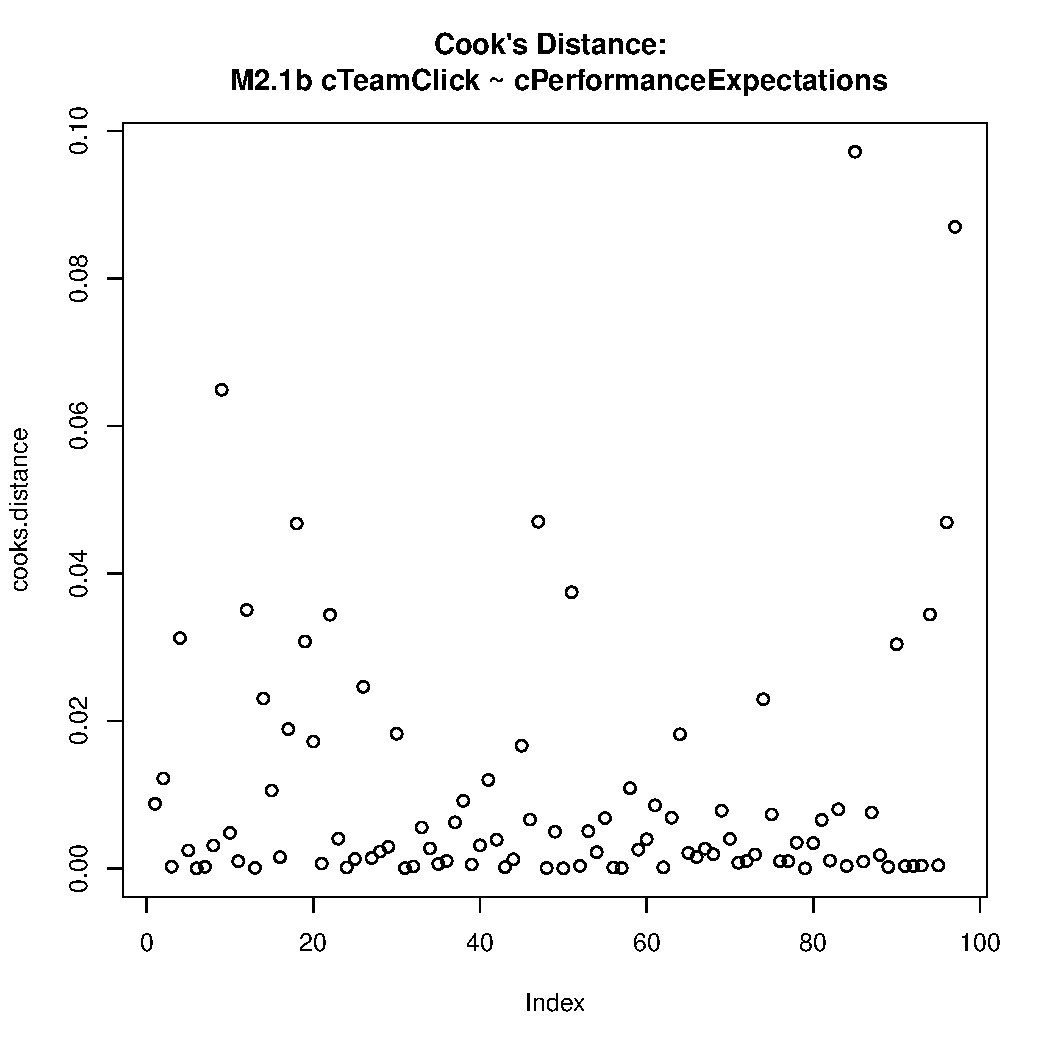
\includegraphics[scale =.4]{images/MLM21bCooksD.pdf}
  \caption{Model Assumptions: M2.1b Team Performance Expectations post-Tournament predicts change in Team Click}
  \label{fig:MLM21bAssumptions}
\end{figure}


\begin{figure}[htbp]
  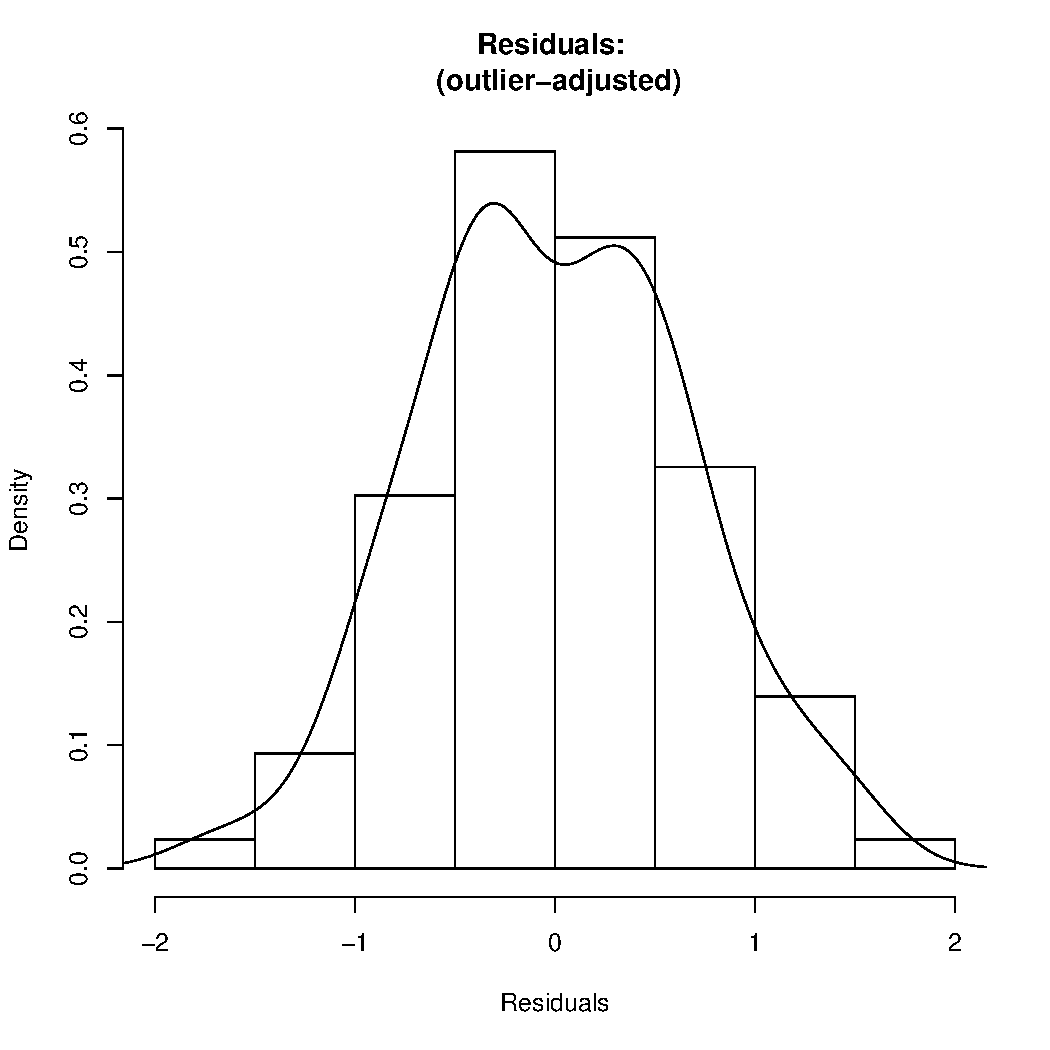
\includegraphics[scale =.4]{images/MLM21bOutHist.pdf}
  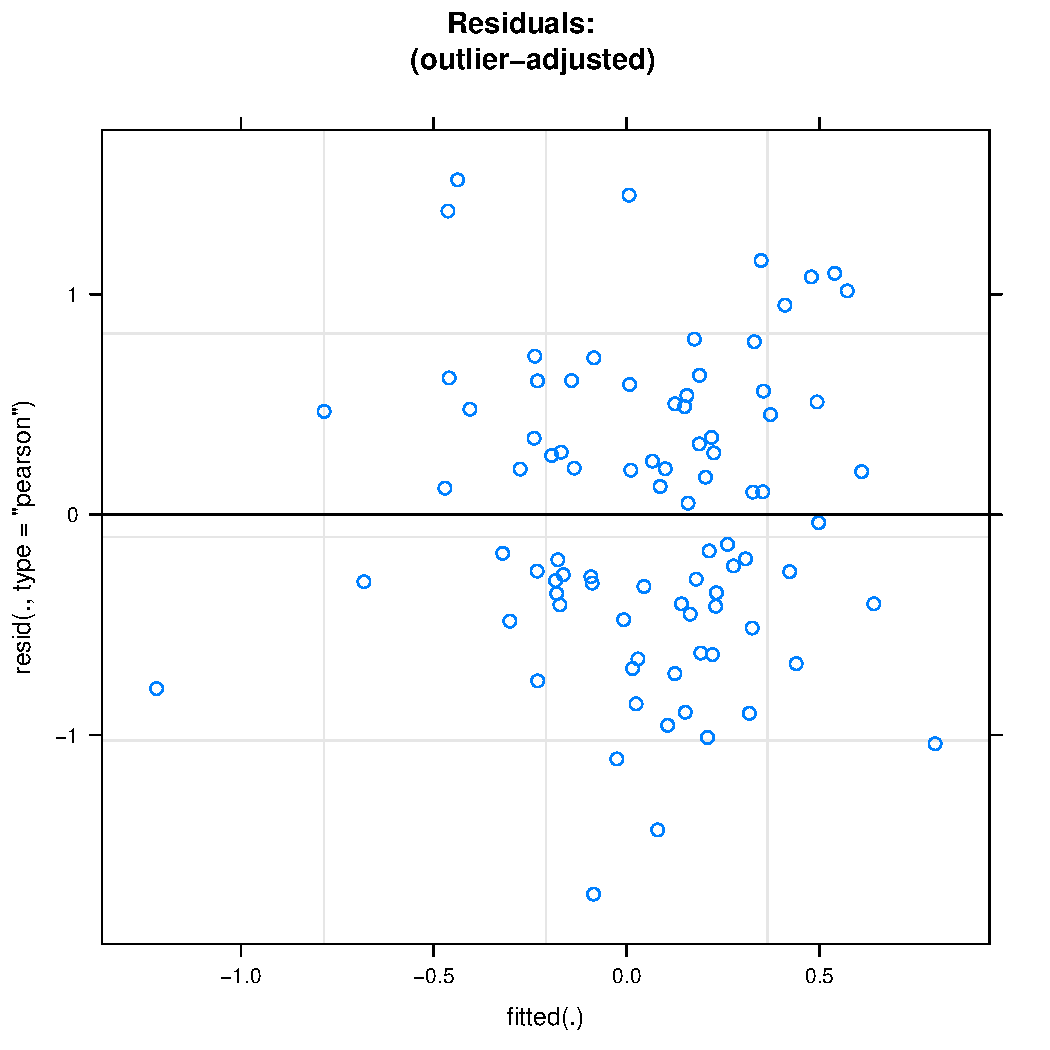
\includegraphics[scale =.4]{images/MLM21bOutScatter.pdf}
  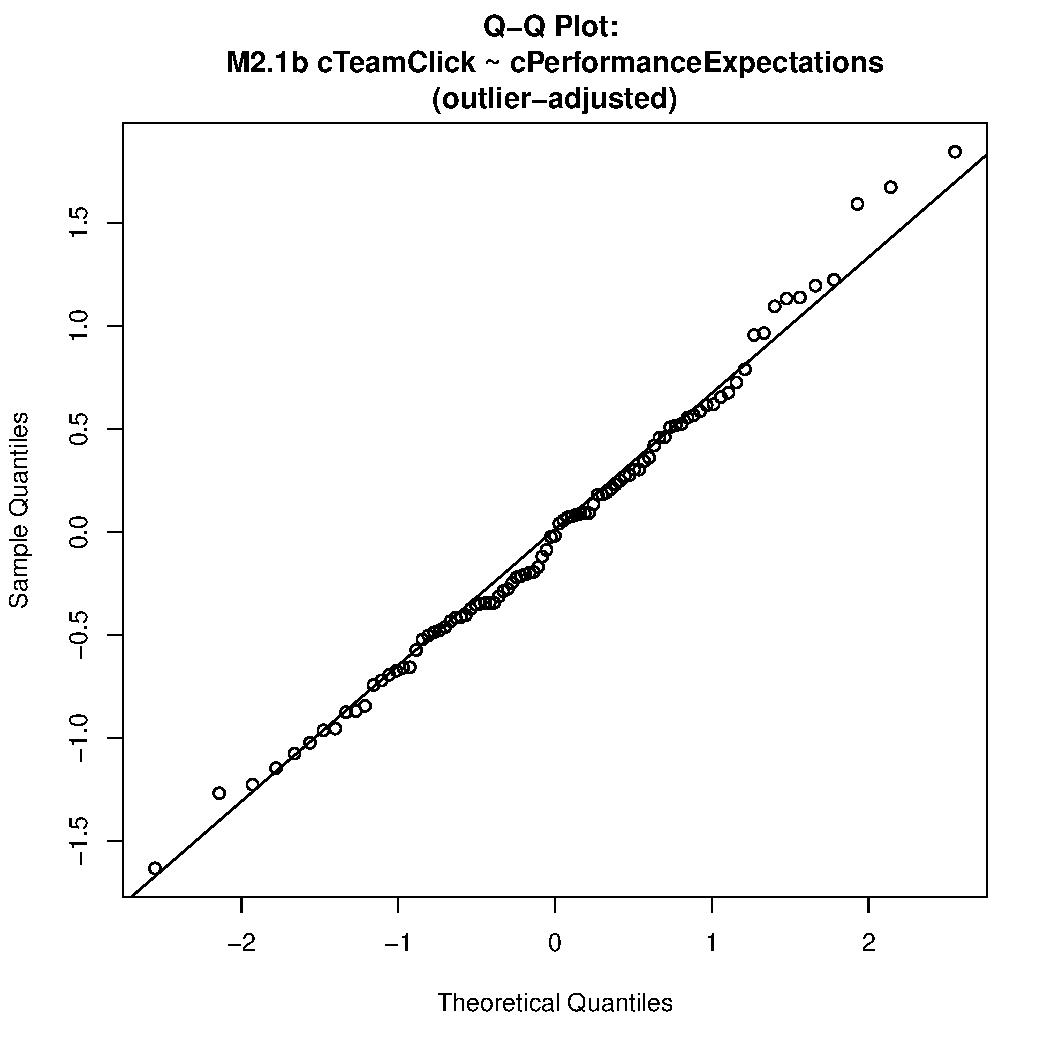
\includegraphics[scale =.4]{images/MLM21bOutQQNorm.pdf}
  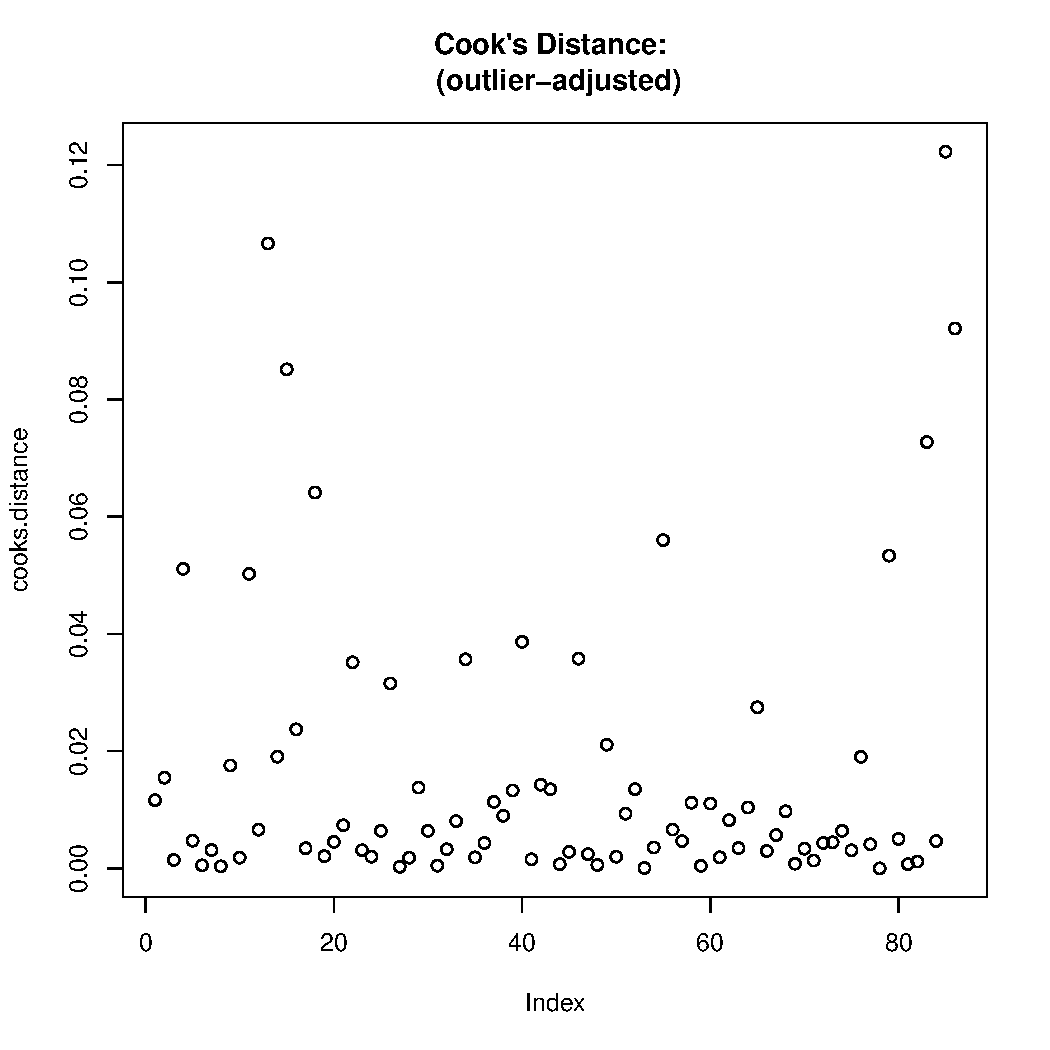
\includegraphics[scale =.4]{images/MLM21bOutCooksD.pdf}
  \caption{Model Assumptions: M2.1b Team Performance Expectations post-Tournament predicts change in Team Click (outliers removed)}
  \label{fig:MLM21bOutAssumptions}
\end{figure}



\begin{figure}[htbp]
  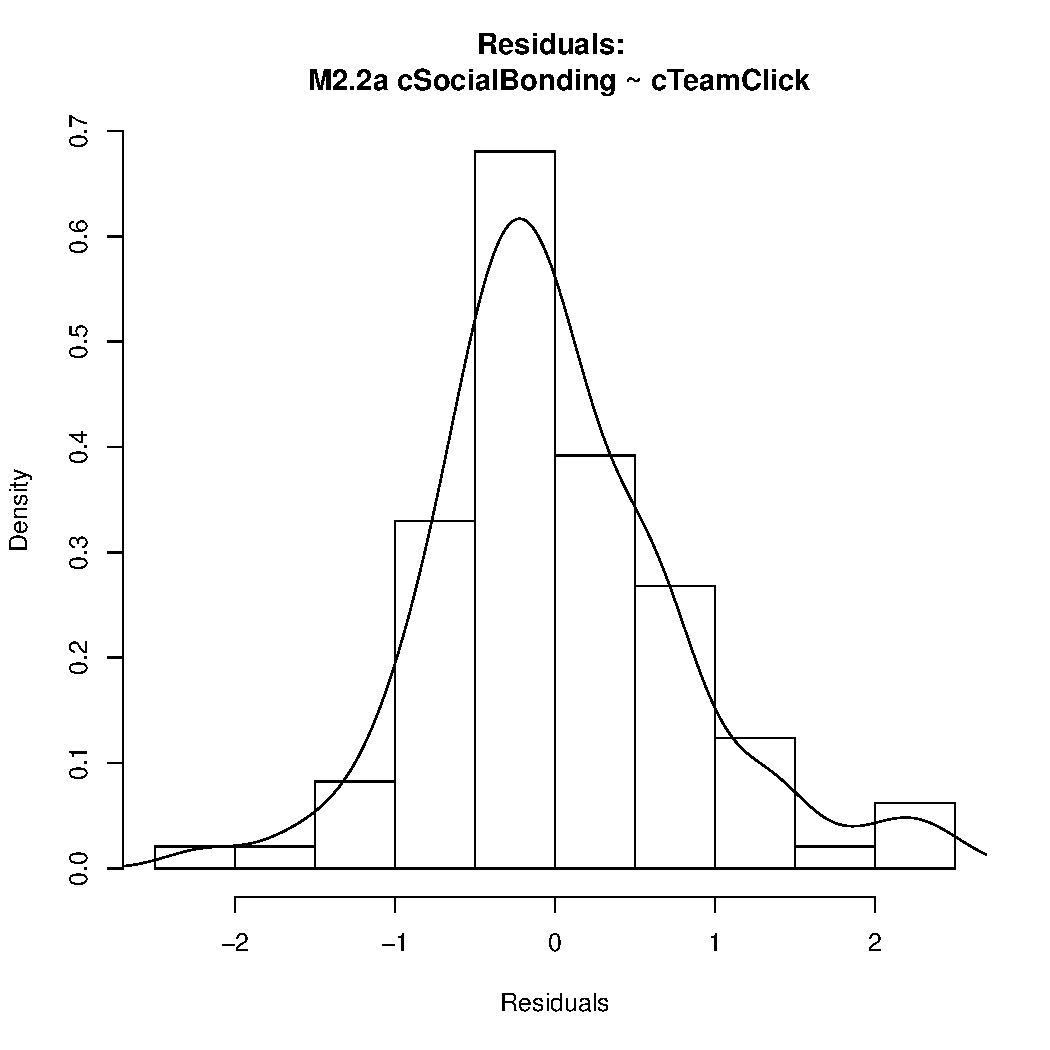
\includegraphics[scale =.4]{images/MLM22aHist.pdf}
  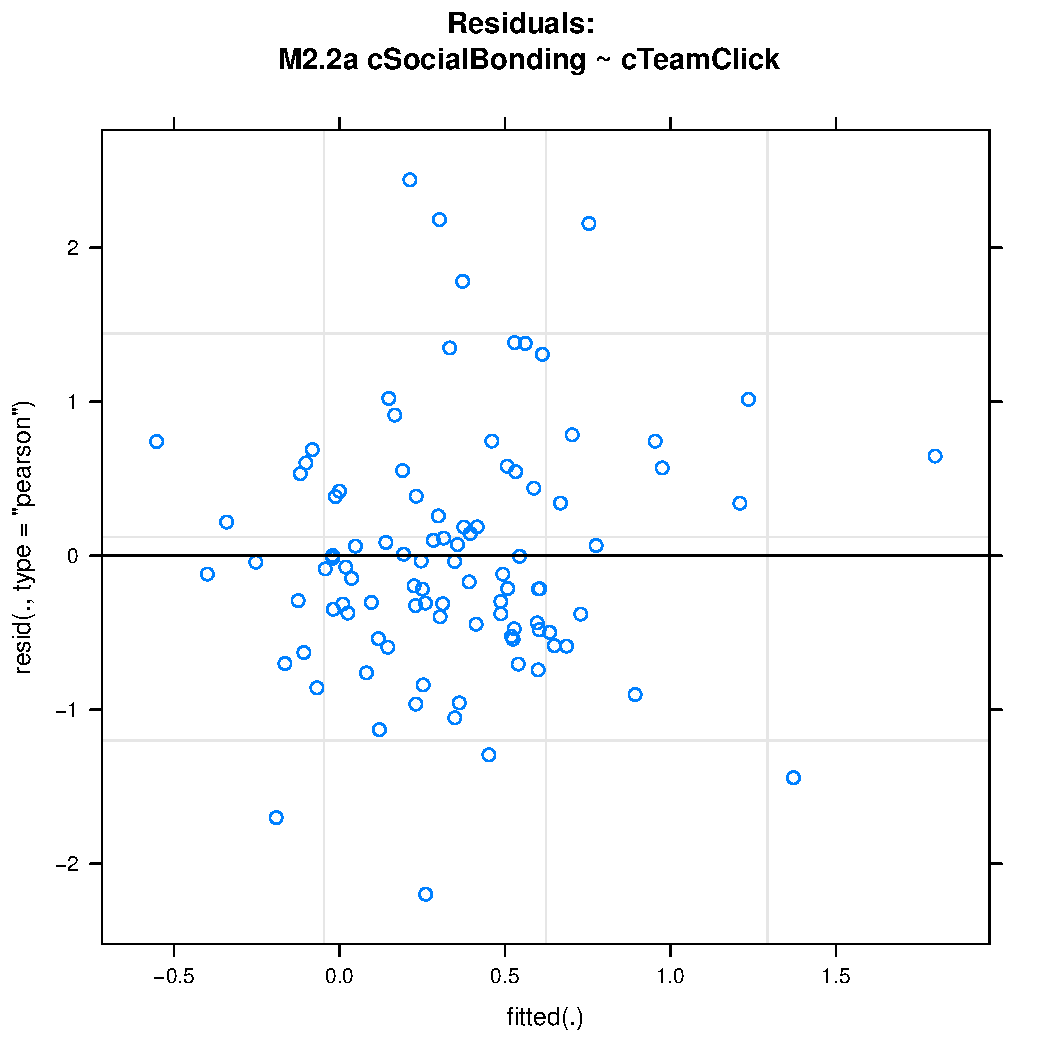
\includegraphics[scale =.4]{images/MLM22aScatter.pdf}
  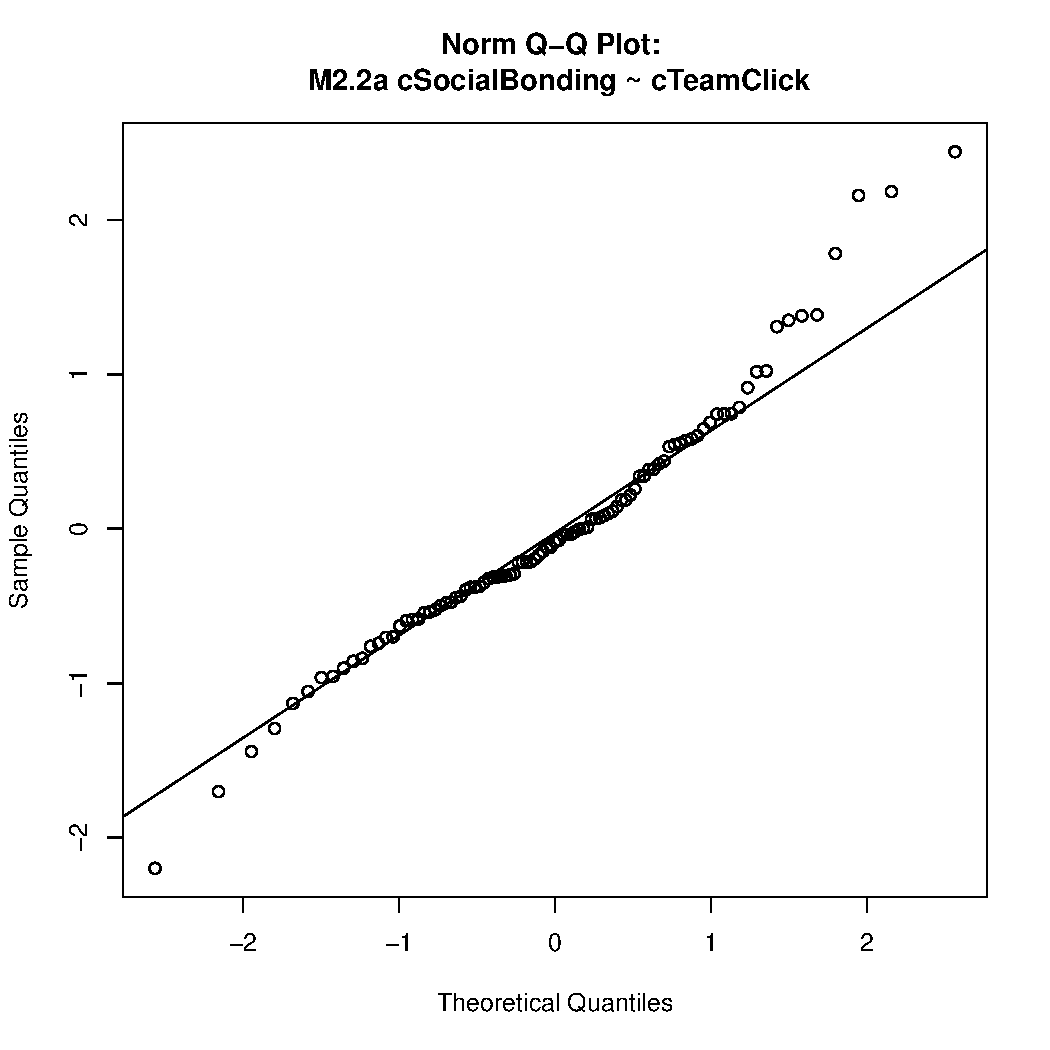
\includegraphics[scale =.4]{images/MLM22aQQNorm.pdf}
  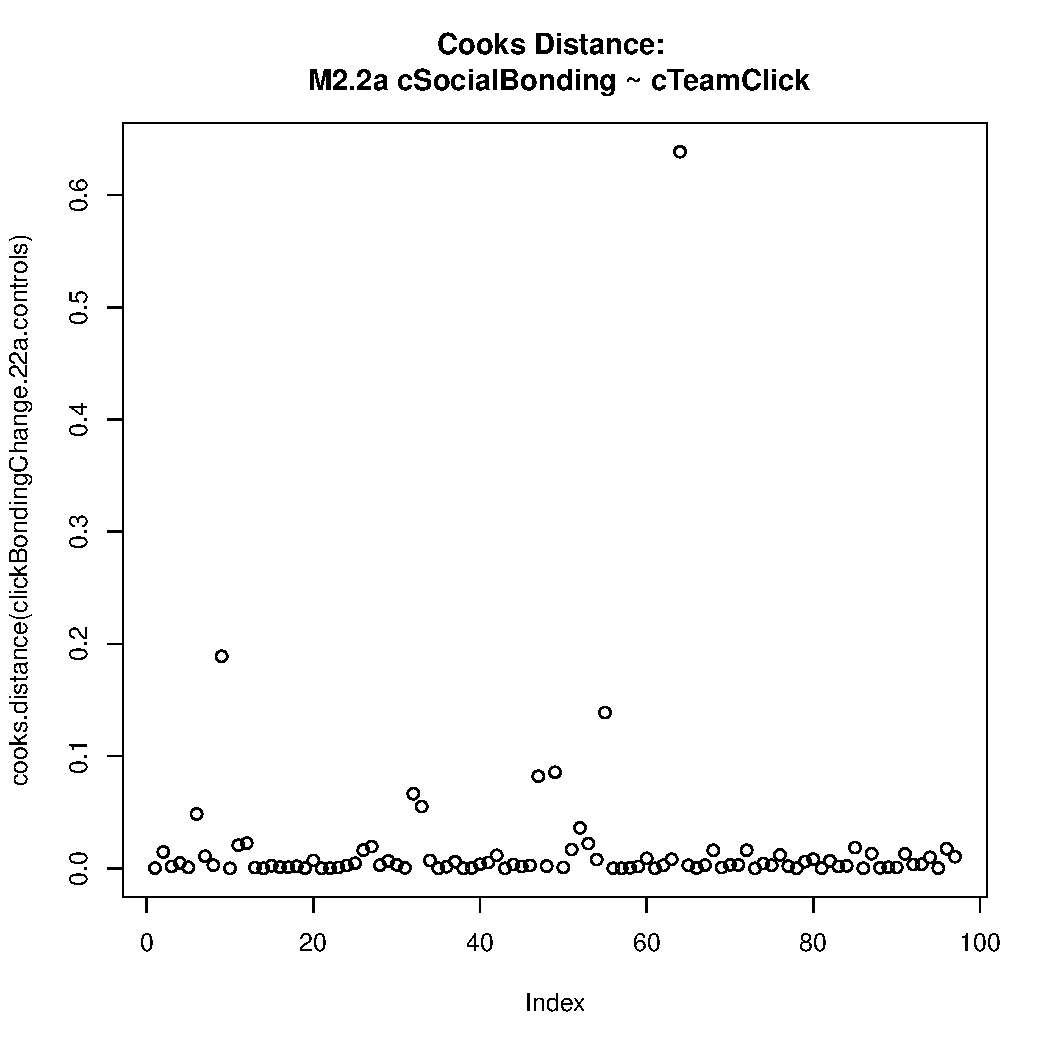
\includegraphics[scale =.4]{images/MLM22aCooksD.pdf}
  \caption{Model Assumptions: M2.2a Change in Team Click predicts change in Social Bonding}
  \label{fig:MLM22aAssumptions}
\end{figure}


\begin{figure}[htbp]
  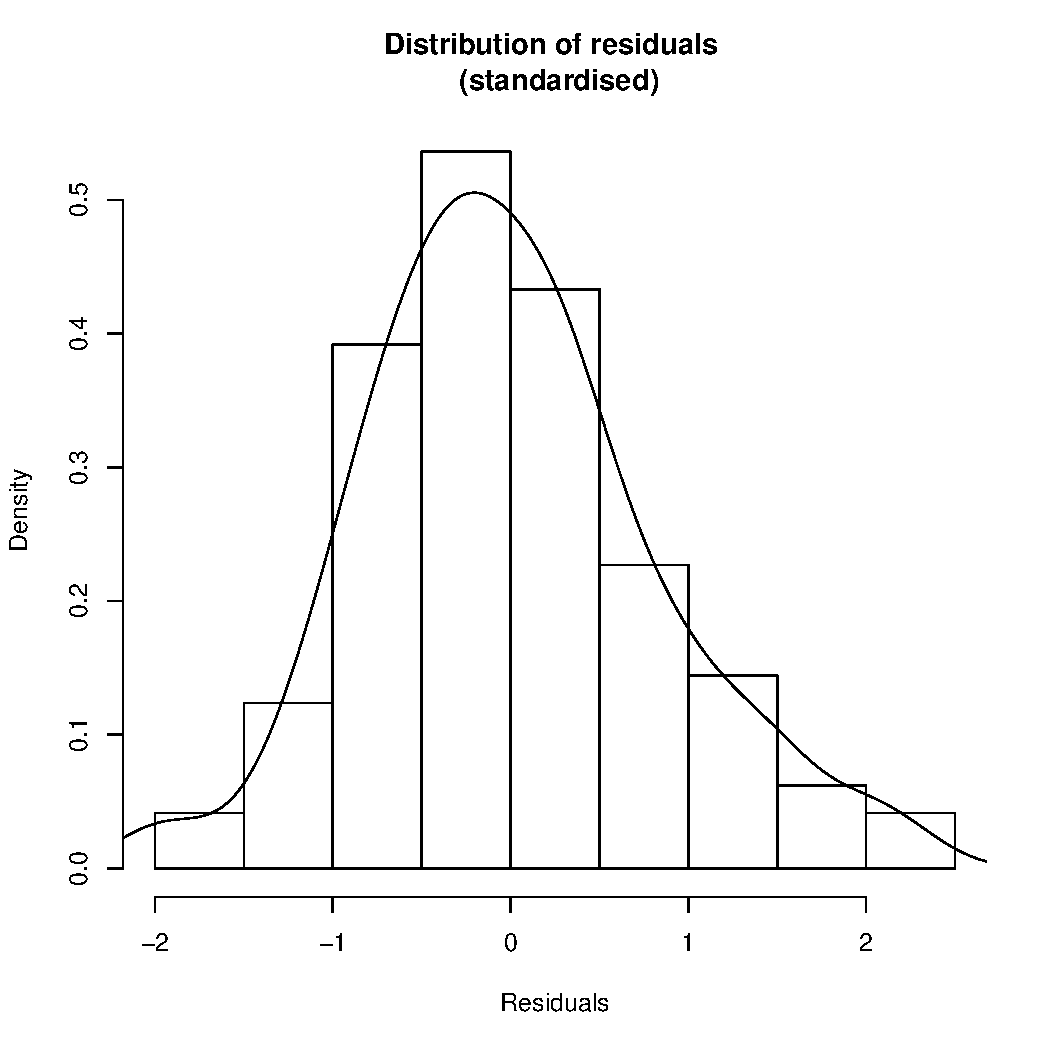
\includegraphics[scale =.4]{images/MLM23aHist.pdf}
  \includegraphics[scale =.4]{images/MLM23aScatter.pdf}
  \includegraphics[scale =.4]{images/MLM23aQQNorm.pdf}
  \includegraphics[scale =.4]{images/MLM23aCooksD.pdf}
  \caption{Model Assumptions: M2.3a Change in Joint Action Success predicts change in Social Bonding}
  \label{fig:MLM23aAssumptions}
\end{figure}



\begin{figure}[htbp]
  \includegraphics[scale =.4]{images/MLM23aHist.pdf}
  \includegraphics[scale =.4]{images/MLM23aScatter.pdf}
  \includegraphics[scale =.4]{images/MLM23aQQNorm.pdf}
  \includegraphics[scale =.4]{images/MLM23aCooksD.pdf}
  \caption{Model Assumptions: M2.3a Change in Joint Action Success predicts change in Social Bonding}
  \label{fig:MLM23aAssumptions}
\end{figure}
